\documentclass[a4paper,9pt]{extarticle}
\newcommand{\budget}{433}

%page geometry
\usepackage[colorlinks,linkcolor=blue,citecolor=blue,urlcolor=blue]{hyperref}
%\usepackage[lmargin=2cm,rmargin=3cm,tmargin=1.25cm,bmargin=1.25cm,includefoot,includehead]{geometry}
\usepackage[lmargin=1.25cm,rmargin=1.25cm,tmargin=1.25cm,bmargin=1.25cm,includefoot,includehead,bottom=1.5cm]{geometry}

%typography
\usepackage[T1]{fontenc}
\usepackage[utf8]{inputenc}
%% Serif Times fonts
\renewcommand{\rmdefault}{ptm} 
%% Sans-serif Arial-like fonts (Helvetica)
\renewcommand{\sfdefault}{phv} 

%text structures
\usepackage{enumitem}
\usepackage{tabu}
\usepackage[dvipsnames]{xcolor}
\usepackage{tcolorbox}
\usepackage{colortbl}
\usepackage{graphicx}
\usepackage{eurosym}
\usepackage{xspace}
\graphicspath{{img/}}

\usepackage{tabularx}
\usepackage{boxedminipage}
\usepackage{spreadtab}

 % \makeatletter
 % 
 % \usepackage{comment}
 % \let\wfs@comment@comment\comment
 % \let\comment\@undefined
 % 
 % \usepackage[todonotes={textsize=scriptsize}]{changes}
 % % uncomment to apply changes
 % %\usepackage[final]{changes}
 % \let\wfs@changes@comment\comment
 % \let\comment\@undefined
 % 
 % \newcommand\comment{%
 % 	\ifthenelse{\equal{\@currenvir}{comment}}
 % 	{\wfs@comment@comment}
 % 	{\wfs@changes@comment}%
 % }
 % 
 % \makeatother
 % \definechangesauthor[name=Pierre Lecomte, color=purple]{PL}

%for added text:
%\added[id=<id>, comment=<comment>]{<new text>}
%for deleted text:
%\deleted[id=<id>, comment=<comment>]{<old text>}
%for replaced text:
%\replaced[id=<id>, comment=<comment>]{<new text>}{<old text>}
%Stating the author’s id and/or a comment is optional.

%Highlight and comment text
%Maybe you want to highlight orcomment some text?
%highlight text:
%\highlight[id=<id>, comment=<comment>]{<text>}
%comment text:
%\comment[id=<id>]{<comment>}


%uncomment if you want to draw a Gantt diagram
\usepackage{pgfgantt}
\usepackage{rotating}


%couleurs ARN 
\definecolor{ANRblue}{HTML}{004d95}
\definecolor{ANRred}{HTML}{FF0000}
\definecolor{ANRpurple}{HTML}{800080}


%physique-chimie
\usepackage{siunitx} %unités en \SI{10}{\micro\metre}
\usepackage[version=3]{mhchem} % Formula subscripts using \ce{}

\usepackage{csquotes}

% %biblio
%\usepackage[backend=biber,style=numeric-comp, language=british,eprint=false, url=false, doi=false, sortcites=true, sorting=none, isbn=false, firstinits=true,maxbibnames=99]{biblatex}
%\renewbibmacro{in:}{%
%  \ifentrytype{article}{}{%
%  \printtext{\bibstring{in}\intitlepunct}}}
%\bibliography{pre-propal-2017}
%\bibliographystyle{plain}

%no month
%\AtEveryBibitem{\clearfield{month}}

%\addbibresource{IEEEabrv.bib}

%lien DOI ou URL si disponible
%\newbibmacro{string+doi}[1]{%
%  \iffieldundef{doi}{%
%    \iffieldundef{url}{#1}{\href{\thefield{url}}{#1}}}{\href{http://dx.doi.org/%\thefield{doi}}{#1}}}

%sur le titre, en couleur
%\DeclareFieldFormat
%  [article,inbook,incollection,inproceedings,patent,thesis,unpublished]
%  {title}{{\textcolor{ANRblue}{#1\addperiod}}}
  

%Our names in bold
\usepackage{xstring}
\usepackage{etoolbox}
%\newboolean{bold}
%% \newcommand{\makeauthorsbold}[1]{%
%% \DeclareNameFormat{author}{%
%%     \setboolean{bold}{false}%
%%     \renewcommand{\do}[1]{\ifstrequal{##1}{####1}{\setboolean{bold}{true}}{}}%
%%     \ifnumequal{\value{listcount}}{1}%
%%     {\ifnumequal{\value{liststop}}{1}%Single author
%%       {\expandafter\ifthenelse{\boolean{bold}}{\textcolor{ANRpurple}{\underline{##1\addcomma\addspace ##4\addcomma\isdot}}}{##1\addcomma\addspace ##4\addcomma\isdot}}
%%       %first author
%%       {\expandafter\ifthenelse{\boolean{bold}}{\textcolor{ANRpurple}{\underline{##1\addcomma\addspace ##4}}}{##1\addcomma\addspace ##4}}}
%%       %last author
%%     {\ifnumless{\value{listcount}}{\value{liststop}}
%%       {\expandafter\ifthenelse{\boolean{bold}}{\addcomma\addspace \textcolor{ANRpurple}{\underline{##1\addcomma\addspace ##4}}}{\addcomma\addspace ##1\addcomma\addspace ##4}}
%%       %middle author
%%           {\expandafter\ifthenelse{\boolean{bold}}{\addcomma\addspace \textcolor{ANRpurple}{\underline{##1\addcomma\addspace ##4\addcomma\isdot}}}{\addcomma\addspace ##1\addcomma\addspace ##4\addcomma\isdot}}%
%%     }%
%% }%
%% }
%% \makeauthorsbold{Cottin-Bizonne,Delanoë-Ayari,Leocmach}

%% %%hack fullcite so that it prints all authors
%% \makeatletter
%% \DeclareCiteCommand{\fullcite}
%%   {\defcounter{maxnames}{\blx@maxbibnames}%
%%     \usebibmacro{prenote}}
%%   {\usedriver
%%      {\DeclareNameAlias{sortname}{default}}
%%      {\thefield{entrytype}}}
%%   {\multicitedelim}
%%   {\usebibmacro{postnote}}
%% \makeatother

% Shrinks space between references
\let\OLDthebibliography\thebibliography
\renewcommand\thebibliography[1]{
  \OLDthebibliography{#1}
  \setlength{\parskip}{0pt}
  \setlength{\itemsep}{0pt plus 0.3ex}
}

\usepackage{titlesec}
\titlespacing*{\section}{0pt}{0.2cm}{0.1cm}
\titlespacing*{\subsection}{0pt}{0.2cm}{0.1cm}
\titlespacing*{\subsubsection}{0pt}{0.2cm}{0.1cm}
\titlespacing*{\paragraph}{0pt}{0.2cm}{0.1cm}

\newcolumntype{P}[1]{>{\raggedright}p{#1}}

%% section title format, in the text and in the table of content
\usepackage{tocloft}

\renewcommand{\cfttoctitlefont}{\color{ANRblue}\normalfont\scshape\bfseries\sffamily\Large}

\usepackage{titlesec}
\titleformat{\section}
{\color{ANRpurple}\normalfont\scshape\bfseries\sffamily\Large}
{\color{ANRpurple}\thesection}{1em}{}
\renewcommand{\cftsecfont}{\color{ANRpurple}\normalfont\scshape\bfseries\sffamily\large}

\titleformat{\subsection}
{\color{ANRblue}\normalfont\scshape\bfseries\sffamily\large}
{\color{ANRblue}\thesubsection}{1em}{}
\renewcommand{\cftsubsecfont}
{\color{ANRblue}\normalfont\scshape\bfseries\sffamily}

\titleformat{\subsubsection}
{\color{ANRpurple}\normalfont\bfseries\sffamily}
{\color{ANRpurple}\thesubsubsection}{1em}{}
\renewcommand{\cftsubsubsecfont}
{\color{ANRpurple}\normalfont\bfseries\sffamily\small}

\titleformat{\paragraph}[runin]
{\color{ANRblue}\normalfont\sffamily}
{\color{ANRblue}\theparagraph}{0em}{}

\newcommand{\secfont}{\noindent\color{ANRblue}\normalfont\sffamily}

\newcommand{\F}{\textsc{Faust}}
\newcommand{\PP}{FAST} 

%titre, acronyme, défi, instrument
\newcommand{\myacro}[0]{\PP}
\newcommand{\mytitle}[0]{\myacro: Fast Audio Signal-processing Technologies on FPGA}
\newcommand{\projectname}[0]{\PP}
\newcommand{\mydomain}[0]{transversaux}
\newcommand{\myinstrument}[0]{PRC}
\author{\hline \textbf{Partners} \\ Grame -- Centre National de Création Musicale (CNCM) \\ CITI -- Institut National de Sciences Appliquées de Lyon (INSA) \\ LMFA -- École Centrale de Lyon \vspace{0.3cm} \\ \textbf{Coordinator} \\ Romain Michon, GRAME-CNCM, Lyon \\ \href{mailto:michon@grame.fr}{\texttt{michon@grame.fr}} \hspace{0.8cm} \url{https://ccrma.stanford.edu/~rmichon}\\ \hline
}

%% Headers
\usepackage{fancyhdr}
\pagestyle{fancy}
%\fancyhfoffset[re]{4cm}
\lhead{{\myacro} -- Coordinateur : Romain Michon (GRAME-CNCM)\\ \myinstrument{} -- Domaines \mydomain{}\\CE38 -- Révolution numérique : rapports au savoir et à la culture }
\rhead{{\LARGE\textcolor{ANRblue}{AAPG ANR 2020}}\\ Aide prévisionnelle : {\budget}K\euro\\Durée : 42 mois}
\renewcommand{\headrulewidth}{0pt}

\lfoot{}
\cfoot{}
\rfoot{\thepage}%/\pageref{LastPage}} 




\title{\vspace{-\baselineskip}\Huge{}\mytitle}
\date{PRC -- Full Proposal\\Domaines transversaux\\
CE38 (Axe 8.6.) Révolution numérique : rapports au savoir et à la culture \vspace{\baselineskip} \\ \textbf{Keywords:} Approche numérique à la création artistique, Traitement audio-numérique ultra-basse latence, Programmation de haut niveau, Acoustique virtuelle \\}

\newcommand{\content}[1]{\emph{#1}\\} 


\begin{document}
\maketitle
\thispagestyle{fancy}

\begin{center}
\begin{tabular}{c | c c | c | c}
\multicolumn{5}{c}{\textbf{Persons Involved In the Project}}\\
\hline
\hline
\textbf{Partner} & \multicolumn{2}{c|}{\textbf{Individual}} & \multicolumn{2}{c}{\textbf{Role, Responsibility, and Effort (in P.m.)}} \\
\hline
Grame & Romain Michon & Researcher & Project coordinator and leader & 10 \\ 
& & & of WP0, WP3, and WP4 \\
\hline
Grame & Yann Orlarey & Researcher & Contributor to WP1 and WP2 & 5 \\
\hline
Grame & Stéphane Letz & Researcher & Leader of WP1 & 8 \\
\hline
Grame & (\textit{To be hired}) & Engineer & Contributor to WP3 & 12 \\
\hline
Grame & (\textit{To be hired}) & Intern & Contributor to WP4 & 6 \\
\hline
CITI & Tanguy Risset & Professor & Leader of WP2 & 13 \\
\hline
CITI & Florent de Dinechin & Professor & Contributor to WP0, WP1, and WP2 & 11 \\
\hline
CITI & (\textit{To be hired}) & PhD Student & Contributor to WP0, WP1, WP2, & 36 \\ 
& & & WP3, WP4, WP5, and WP6 \\
\hline
LMFA & Pierre Lecomte & Associate Professor & Leader of WP5 and WP6 & 11 \\
\hline
LMFA & Marie-Annick Galland & Professor & Contributor to WP0, WP5 and WP6 & 6 \\
\hline
LMFA & Sébastien Ollivier & Associate Professor & Contributor to WP0 and WP4 & 4 \\
\hline
LMFA & (\textit{To be hired}) & Postdoc & Contributor to WP6 & 18 \\ 
\hline
LMFA & (\textit{To be hired}) & Intern & Contributor to WP5 & 6 \\
\end{tabular}
\end{center}

% FULL_PROPOSAL
% \tableofcontents

\section*{Evolution Since the Pre-Proposal}
\addcontentsline{toc}{section}{Evolution Since the Pre-Proposal}

The following modifications were made since the pre-proposal: (1) We reinforced the links between the project and SHS by highlighting in the context of the arts the applications of the tools that will be developed. In particular, a studio/rehearsal space with a modular acoustic featuring events open to the public will be implemented at LMFA. (2) We tried to make the essence of the proposal higher-level and less technical, taking the pre-proposal reviewer's comments into account. (3) Workpackages were reorganized to carry out all the hardware-related tasks before the work around artificial reverberation and active noise control. We also added some overlap between the two workpackages related to artificial reverberation and active noise control. (4) The overall budget of the project has been increased by 5\% to take into account additional equipment costs related to new tasks in some workpackages which consequently resulted in a 5\% increase of the requested funding. (5) The content of each workpackage is now thoroughly described and we provided additional technical details about the methodology that will be used for each task. 

\section{Context, Positioning, and Objectives}

Embedded systems for audio and multimedia are increasingly used in the arts and culture (e.g., interactive systems, musical instruments, virtual and augmented reality, artistic creation tools, musical composition and performance, etc.). However, programming them can be out of reach to artists, creators, or non-specialized engineers. In parallel with the emergence of the ``maker culture,''\footnote{\url{https://makerfaire.com/maker-movement} (All URLs were verified on May 1, 2020).} progress have been made to make these types of systems more accessible, bringing more flexibility in digital approaches to artistic creation. For instance, the Arduino platform\footnote{\url{https://www.arduino.cc}} greatly simplified the programming process of microcrontrollers. Similarly, Domain Specific programming Langages (DSL) such as \F{}\footnote{\F{} is a DSL for real-time audio signal processing primarily developed at GRAME-CNCM and by a worldwide community. \F{} is based on a compiler ``translating'' DSP specifications written in \F{} into a wide range of lower-level languages (e.g., C, C++, Rust, Java, WASM, LLVM bitcode, etc.). Thanks to its ``architecture'' system, generated DSP objects can be embedded into template programs (wrappers) used to turn a \F{} program into a specific ready-to-use object (e.g., standalone, plug-in, smartphone app, webpage, etc.). } 
\cite{Orlarey2009} facilitated the implementation of real-time audio Digital Signal Processing (DSP) algorithms.

However, many limitations remain, especially for real-time applications where latency plays a crucial role (e.g., efficient active control of sound where audio processing should be faster than the propagation of sound \cite{elliott2000signal}, digital musical instruments playability \cite{Lago2004}, digital audio effects, etc.). While latency can be potentially reduced on ``standard'' computing platforms such as personal computers based on a CPU (Central Processing Unit), going under the ``one millisecond threshold'' is usually impossible because of buffering.

FPGAs (Field Programmable Gate Arrays) can help solve this problem as well as most of the limitations of traditional computing platforms used for musical and artistic applications. These chips are known for their high computational capabilities \cite{Choi2013,Pfeifle2012} and very low-latency performances \cite{Verstraelen2014}. They also provide a large number of GPIOs (General Purpose Inputs and Outputs) which can be exploited to implement modern real-time multi-channel processing algorithms (e.g., sound fields capture using a very large number of digital microphones \cite{salze2019new}, active sound control over a large spatial region \cite{Zhang2018}, etc.). 

But FPGAs remain extremely complex to program, even with state-of-the-art high-level tools,\footnote{FPGAs are configured/programmed using a Hardware Description Language (HDL) such as VHDL or Verilog. The learning curve and the electrical engineering skills required to master these types of environments make them out of reach to the real-time audio DSP community. Solutions exist to program FPGAs at a higher level (i.e., LabVIEW: \url{https://www.ni.com/fr-fr/shop/labview.html}, Vivado HLS: \url{https://www.xilinx.com/HLS}, etc.), but none of them is specifically dedicated nor adapted to real-time audio DSP.} making them largely inaccessible to musicians, digital artists and makers communities.
There are currently only a few examples of professional FPGA-based real-time audio DSP systems (i.e., Antelope Audio,\footnote{\url{https://en.antelopeaudio.com}} Korora Audio,\footnote{\url{https://www.kororaaudio.com}} etc.) and in these applications, FPGAs are dedicated to a specific task, limiting creativity and flexibility.

\begin{figure}[h]
  \centering
  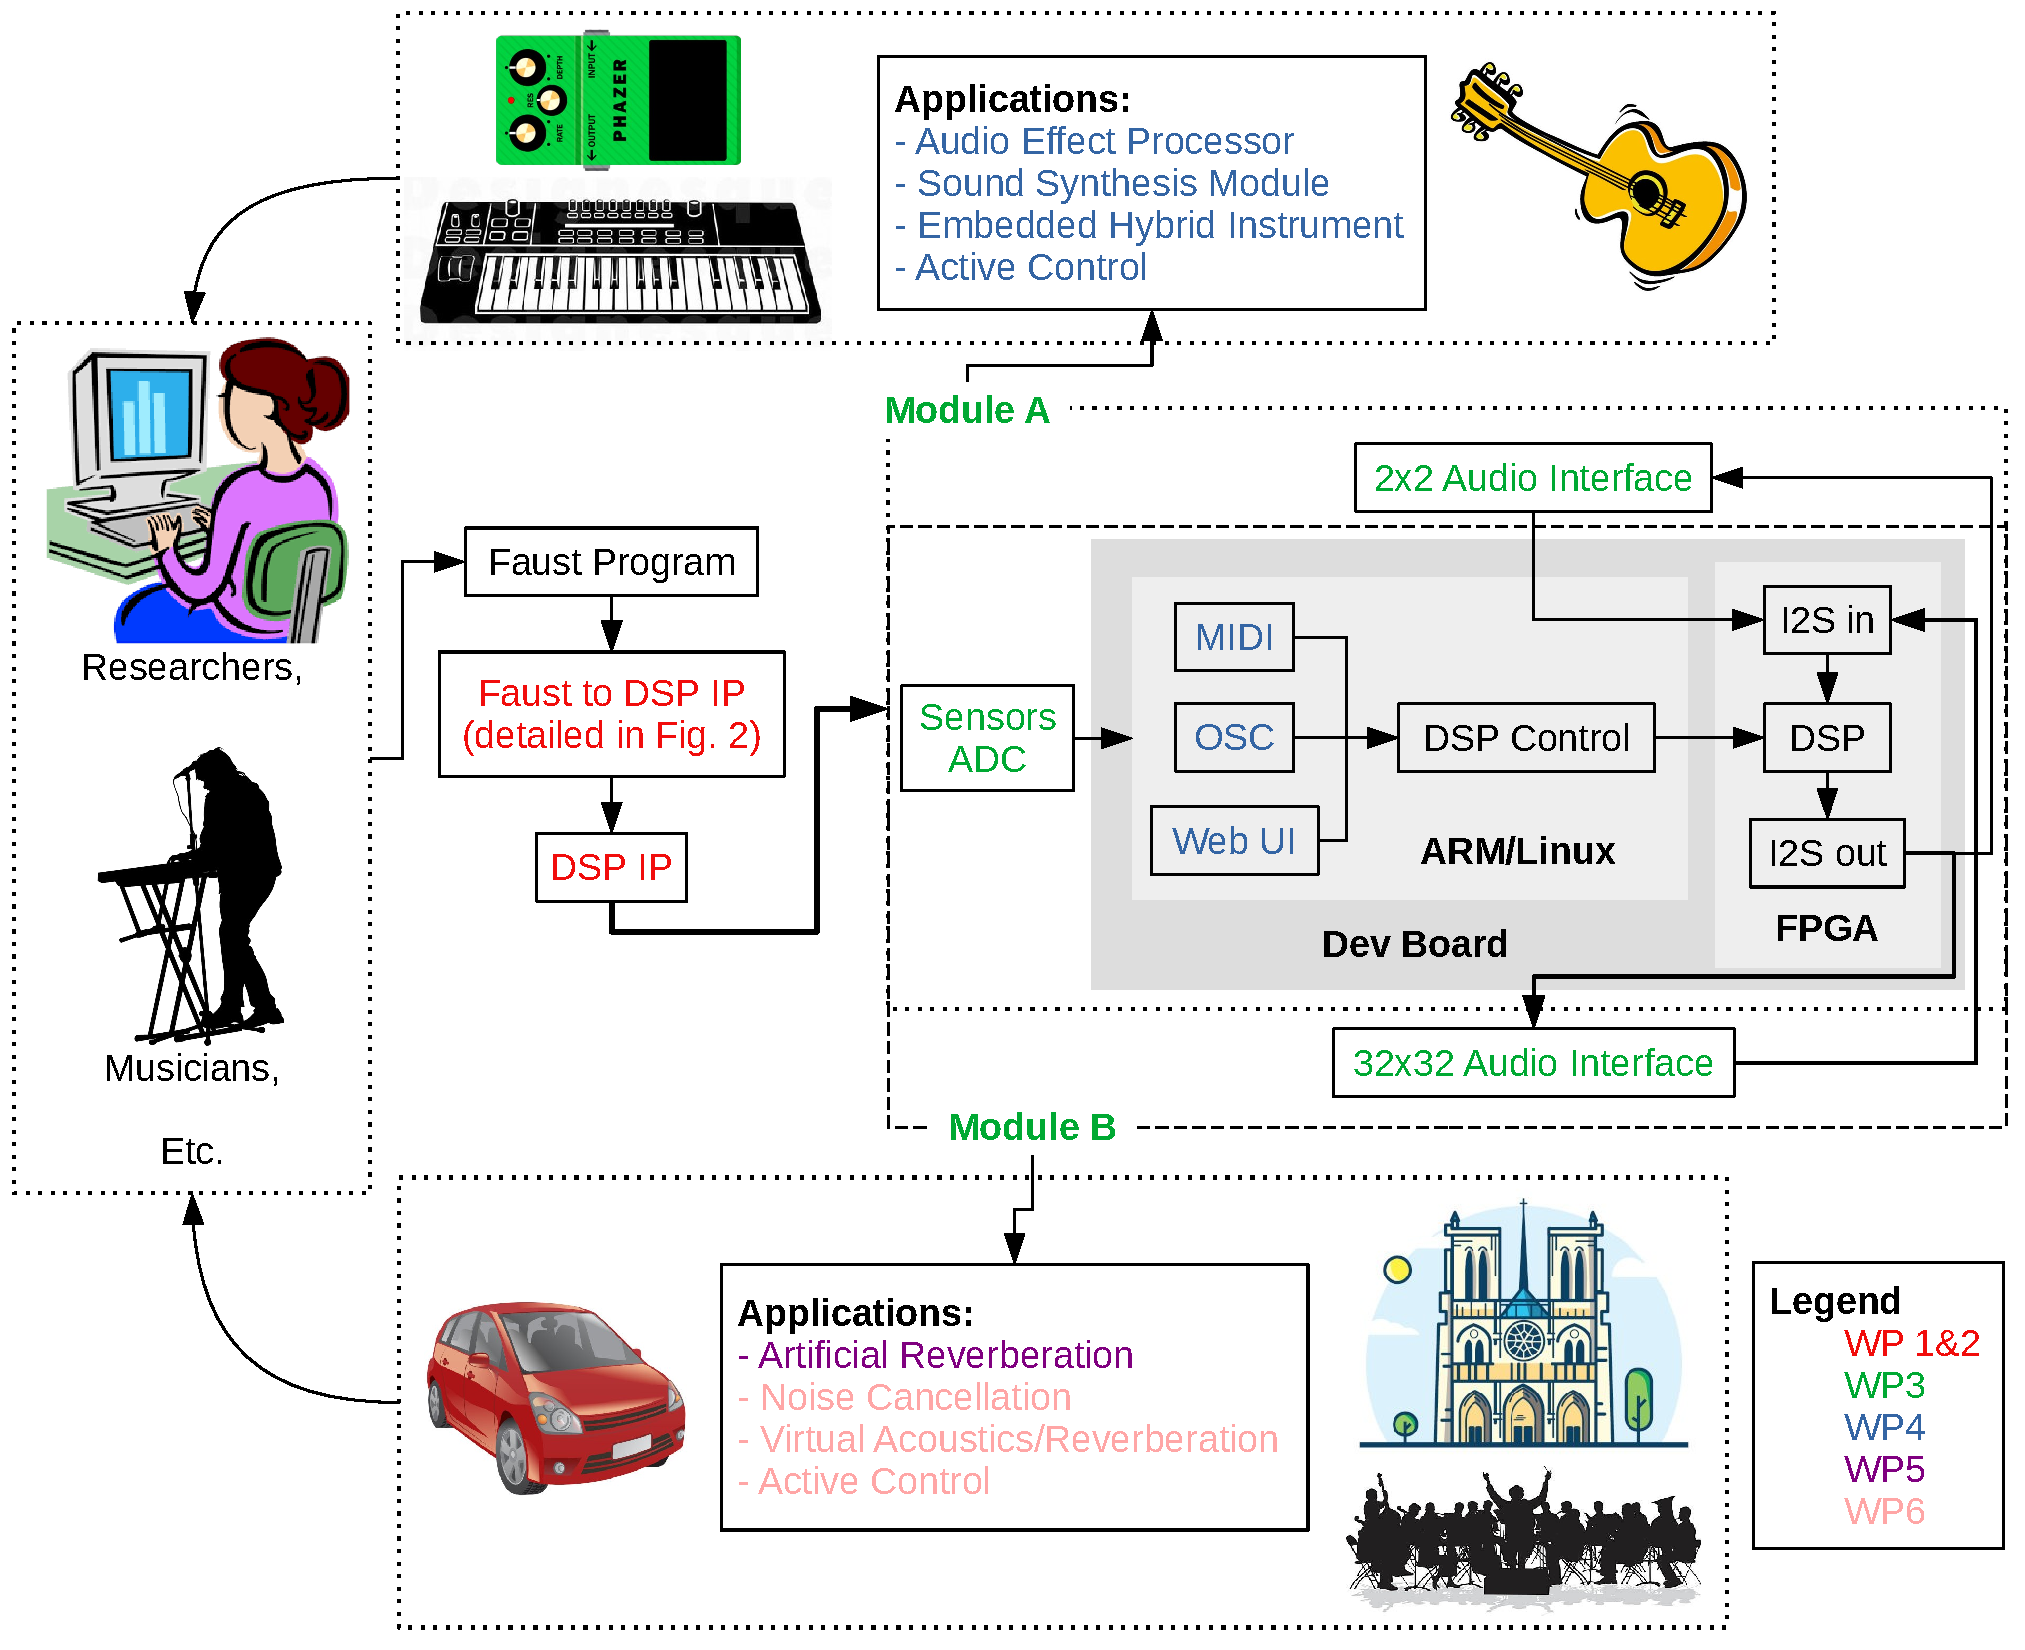
\includegraphics[width=13cm]{img/overview}
  \caption{\PP{} overview.}
  \label{fig:overview}
\end{figure}

\subsection{Objectives and Research Hypothesis}

The \PP{} project was thought to overcome the aforementioned difficulties (i.e., low latency, computing capacity, multi-channel, and ease of programming). \textbf{The goal of \PP{} is to design an FPGA-based platform for multichannel ultra-low-latency audio Digital Signal Processing (DSP) programmable at a high-level with \F{}} and usable for various applications ranging from sound synthesis and processing to active sound control and artificial sound field/room acoustics. In addition to that, we then plan to use this tool to: 

\begin{itemize}
  \itemsep0em
  \item design a programmable sound processing/synthesizer module for musicians, artists, and makers; 
  \item actively modify the acoustical properties of acoustic musical instruments and create ``smart/hybrid instruments;''
   \item create a studio/rehearsing space with an adaptive acoustic.
\end{itemize}

\PP{} will gather the strengths of GRAME-CNCM\footnote{\url{http://grame.fr}} (\F{}, compilation, musical audio applications, dissemination/mediation, professional music production), CITI\footnote{\url{http://www.citi-lab.fr}} at INSA Lyon (FPGA, DSP, fixed-point processing with FloPoCo\footnote{\url{http://flopoco.gforge.inria.fr}}), and LMFA\footnote{\url{http://lmfa.ec-lyon.fr}} at École Centrale de Lyon (acoustics, DSP, artificial reverberation, active control).

The main objective of \PP{} is to \textbf{develop a new \F{} architecture backend for FPGA-based platforms}. One of the challenges here is the optimization of the module generated by \F{}. The real breakthrough will be obtained with the use of two recent technologies in the \F{} compilation workflow: {\bf $(i)$ High Level Synthesis} (HLS) for compiling \F{} program to VHDL and {\bf $(ii)$ fixed-point support} in the code generated by the \F{} compiler, building on the expertise developed at CITI around the FloPoCo project. Eventually, we aim at generating VHDL code directly from the \F{} compiler. 

This type of system has a wide range of applications in multiple domains. As mentioned earlier, music technology is in high demand for low latency because it helps increasing the playability of musical instruments on stage. Hence, the platform developed as part of \PP{} will be used to design programmable digital musical instruments and effect processors. In that context, the computational power of the FPGA will be exploited to run complex algorithms (e.g., physics-based models of musical instruments \cite{Bilbao2009}, modal reverbs \cite{Abel2009}, etc.) that are too costly to run on a traditional platform (i.e., laptop, etc.). GRAME-CNCM has decades of experience in that domain. 

We plan to \textbf{implement two hardware/software audio DSP modules based on the platform} implemented in \PP{}. One will target the makers and music technology communities and will provide a stereo input and output as well as GPIOs for sensors. The other will target active acoustic control and spatial audio applications by providing 32 audio inputs and outputs.

One of the main field of application for the platform that we plan to develop as part of \PP{} is active control of acoustical spaces (e.g., noise cancellation in rooms, car passenger compartment, etc.) and virtual room acoustics (e.g., to apply the acoustical properties of a space to another, etc.). Sound field rendering systems are in high demand for low audio latency (i.e., to beat acoustical waves traveling at the speed of sound in the air) and high computational power (i.e., to implement Finite Difference Time Domain: FDTD schemes \cite{Bilbao2009}). While FPGAs have been used in the past for this type of applications \cite{Tan2019}, there is a lack for a high-level tool to program and implement these types of algorithms. Similarly, FPGAs should allow to run in real-time room acoustics simulation algorithms such as modal reverbs \cite{Abel2019} in the time domain, which is not currently possible on regular computers. LMFA École Centrale has a lot of experience in these domains and a wide range of equipment at its disposal (e.g., sound field array/listening room, etc.) that will be used/adapted to this purpose. We plan to \textbf{prototype real-world examples of room acoustics simulation/modifications} that could then be used in a concert setting. Such experiments have been attempted in the past at the Center for Computer Research in Music and Acoustics (CCRMA)\footnote{\url{https://ccmra.stanford.edu}} at Stanford University that is indirectly related to \PP{} thanks to Romain Michon's affiliation. In particular, the acoustics of the Hagia Sophia cathedral in Istanbul has been recreated in Stanford's Bing Concert Hall for a series of concerts centered around the idea of ``archeoacoustics'' \cite{Abel2009}. The platform that we plan to implement as part of \PP{} will be used to take this type of system to a completely different level. Hence, we plan to organize events centered around these concepts with the help of GRAME-CNCM music production department. In particular, \textbf{we will design a system to recreate the acoustics of various landmarks from the Lyon area in LMFA's listening room to turn it into an immersive studios} where small events open to the public will be organized. 

Finally, applications around active control are not limited to acoustical spaces. Musical instrument acoustics/digital lutherie are increasingly using these types of techniques \cite{Zhang2018} not to mention industrial applications outside of the field of audio (e.g., aircraft jet engine vibration control, etc.) which would be easily reachable thanks to LMFA's expertise in these domains \cite{salze2019new}.

\subsection{Positioning In Relation to the State of the Art}

\subsubsection{Domain Specific Languages for Real-Time Audio DSP}

While there exists many high-level standard programming languages providing libraries/environments for asynchronous signal processing (e.g., MATLAB, Python, etc.), real-time DSP is usually programmed through C/C++ or even lower level paradigms. Nonetheless, several languages targeting real-time signal processing applications such as Kronos \cite{norilo2015kronos}, Arrp \cite{leben2016arrp}, Stride \cite{tilbian2017stride}, CSOUND \cite{lazzarini2016csound}, and more recently SOUL\footnote{\url{https://soul.dev/}} have been available for many years. \F{} \cite{Orlarey2009} is part of that category as well and can be regarded as the main alternative to C/C++ for real-time audio applications. By allowing us to target an unparalleled number of systems and platforms, it is now considered as a standard both in the industry and in academia. We plan to take advantage of \F{}'s accessibility, versatility, and ease of use as part of \PP{} to facilitate the programming of FPGAs. 

One important step is to enable fixed-point data computation in \F{}-generated code. Indeed, sound samples are essentially fixed-point data, and using floating-point for sound processing is inherently inefficient. It does make sense on CPUs which include expensive floating-point units anyway, but the main reason why floating-point is used for sound processing is that it is convenient, relieving the designer from having to think about the range and accuracy of data in a program.
In \PP{}, we intend to provide an accessible programming paradigm while offering better efficiency, thanks to a compiler that automatically determines fixed-point formats.

\subsubsection{Ultra-Low-Latency Signal Processing}
\label{subsubsec:lowlatency}

Audio latency is a central concern when it comes to digital audio \cite{Lago2004}. There are typically two main sources of latency on digital audio systems: buffering at the software/computation level and Digital to Audio Converters (DAC) themselves (mostly because of signal reconstruction filters). While ultra-low-latency ($50 \mu s$) audio ADCs/DACs such as the Analog Devices ADAU177\footnote{\url{https://www.analog.com/en/products/adau1777.html}} can be found on the market, achieving ultra-low-latency can be relatively hard on the software and computational side. 

Various systems both in the industry and in academia have been targeting low audio latency through the use of different hardware solutions. The most approachable ones are embedded Linux systems using dedicated hardware and running audio DSP outside of the operating system. The BELA \cite{mcpherson2015} and the Elk\footnote{\url{https://elk.audio/}} are the only two members of this family. They target the  Beagle Bone,\footnote{\url{https://beagleboard.org/}} and the Raspberry Pi\footnote{\url{https://www.raspberrypi.org/}} respectively. This type of system can achieve relatively low-latency with buffer sizes as low as 8 samples.

Microcontrollers have been used more and more in recent years for sound synthesis and processing because of their increasing power. The Teensy\footnote{\url{https://www.pjrc.com/teensy/}} \cite{Michon2019} and the ESP32\footnote{\url{https://www.espressif.com/en/products/hardware/esp32/overview}} \cite{Michon2020} are good examples of such systems. Thanks to their lightness (e.g., no OS), their latency performances are similar to that of dedicated/specialized embedded Linux systems (i.e., buffer size of 8 samples as well).  

Digital Signal Processors (DSPs) can target even lower latency with buffer sizes as low as 4 samples and provide tremendous amounts of computational power for signal processing applications. They usually target engineers making them less approachable than the other types of systems mentioned in this section. Additionally, many of them don't provide native support for floating-points, further increasing the complexity of their programming. The Analog Devices SHARC Processor\footnote{\url{https://www.analog.com/en/products/processors-dsp/dsp/sharc.html}} is a leader on the market and it can be used as a prototyping system through the SHARC Audio Module.\footnote{\url{https://www.analog.com/en/design-center/evaluation-hardware-and-software/evaluation-boards-kits/sharc-audio-module.html}} It also provides an official \F{} support.\footnote{\url{https://wiki.analog.com/resources/tools-software/sharc-audio-module}} Cheaper/more lightweight DSP-based platforms such as the ESP32 LyraTD\footnote{\url{https://www.espressif.com/en/products/hardware}} are also starting to appear.

The only way to take audio latency one step further down is to use FPGAs, which is what we plan to do in \PP{}.

\subsubsection{FPGAs Programming for  Real-Time Audio Processing}

FPGAs have been used in the field of audio processing for their high computational capabilities \cite{Choi2013,Pfeifle2012,motuk2005implementation,motuk2007design} and very low-latency performances \cite{Verstraelen2014}. Their large number of GPIOs (General Purpose Inputs and Outputs) has also been exploited to implement modern real-time multi-channel processing algorithms (e.g., sound fields capture using a very large number of digital microphones \cite{salze2019new,wavefield}, various signal processors for audio~\cite{AudioMovie,zhang2015design}). The resulting FPGA design are rarely open source. Recently, Vaca et al. presented an open audio processing platform based on the Zybo board~\cite{zyboAudio} for dedicated purpose such as collecting analog frequency of a musical instrument. However, this project was not targeting ultra-low-latency applications.

Programming FPGA is usually done with a hardware description language (VHDL or Verilog). Developing a VHDL IP\footnote{IP stands for Intellectual Property, it is the common denomination for {\em hardware library}, i.e., a circuit design that can be re-used as a software library} is extremely time consuming. Hence, FPGA programmers have two possibilities: re-using existing IPs and assemble them to compose a circuit solving their problem (as proposed by LABVIEW\footnote{\url{https://www.ni.com/fr-fr/shop/labview.html}}), or use High-Level Synthesis to {\em compile} a VHDL specification from a higher-level description.

High Level Synthesis~\cite{HLS} has been referred to for decades as {\em the} mean to enable fast and safe circuit design for programmers. However, the design space offered to a hardware designer is so huge that no automatic tool is able to capture all the constraints and come up with the {\em optimal} solution. Many HLS tools have been proposed (i.e., Pico~\cite{pico}, CatapultC~\cite{catapultC}, Gaut~\cite{gaut}, to cite a few) dedicated to specific target application domains. Most of the existing tools start from a high-level representation that is based on a programming language (C, C++, or Python) which is {\em instrumented} using pragmas to guide the HLS process.

Using HLS today still requires very specific skills~\cite{HLSbook} to write a source description that is correctly processed by HLS tools. For instance, the use of optimized fixed-point arithmetic is mandatory because floating-point arithmetic on FPGA is much more expensive. This problem requires more than simple engineering to be tackled~\cite{volkova:hal-01561052, cairn, sentieysid}.  Using CITI expertise in that domain~\cite{flopoco} will be a major technological breakthough that will enable efficient compilation of \F{} programs on FPGA. We believe that HLS technology has reached a certain maturity and can now be foreseen as a valuable tool for audio designers, DSP engineers and researchers, etc.

In \PP{}, we plan to take this kind of work to the next level by making FPGA platforms more accessible for ultra-low-latency multi-channel real-time signal processing applications.

\subsubsection{Active Control of Musical Instruments}

Since the 90's, different active control techniques have been successfully applied to the control of hybrid musical instruments in research laboratories, first for percussion and string instruments, and more recently for wind instruments \cite{Benachio-2016,Boutin-2001,meurisse2015experimental,Meurisse2015-Mute}. The use on stage of augmented instruments with integrated sensors and actuators and real-time control of the resonances using computers have shown new musical perspectives.
Brass mutes based on active sound control such as Yamaha's Silent Brass\footnote{\url{https://fr.yamaha.com/fr/products/musical\_instruments/winds/silent_brass/index.html}} and actively controlled acoustic guitars (i.e., HyVibe\footnote{\url{https://www.hyvibe.audio/smart-guitar/}}) are now available on the market.
However, signal processing in these instruments is much simpler than one would expect from laboratory studies. Actually, the lack of efficient and fast computing capabilities has limited the complexity of control algorithms in smart musical instruments with embedded controllers. The development of hybrid instrument and the wider appropriation of active control techniques by musicians, musical instruments makers, and sound artists will now depend on the availability of easily programmable, affordable, and very fast electronic controllers.

\subsubsection{Artificial Reverberation}

Artificial reverberation can be implemented using a wide range of techniques such as feedback delay networks, waveguide meshes, finite difference scheme, simple combination of IIR filters, and Impulse Responses (IR) convolution \cite{valimaki2012fifty}. The latter has been made more accessible by the increasing power of computers in recent years (it is relatively computationally intensive compared to some of the other methods). It allows us to apply the reverberation of an existing space onto a dry signal by convolving it with the IR of the space \cite{reilly1995convolution}. When recorded with an ambisonic microphone, the IR can be used to recreate the reverberation of a space in 3D using a speaker array. This method has been used in the framework of various projects around ``archeoacoustics'' which partly consists in recreating the acoustical environments of lost or forbidden spaces potentially towards real-time performances. The recreation in Bing Concert Hall at Stanford University of the acoustic of the Hagia Sophia cathedral in Istanbul \cite{Abel2009} is a good example of that. As part of \PP{}, we plan to establish a catalog of 3D IRs of landmarks from the Lyon area to recreate their acoustics in LMFA's listening room.  

Convolution reverbs have been taken to another step recently by introducing the concept of ``modal reverb'' \cite{Abel2019} where convolution is carried out in the time domain instead of the frequency domain by using a bank of resonant bandpass filters taking advantage of the principle of modal decomposition \cite{Adrien91}. This approach is much more controllable since it gives access to the parameters of all the filters used in the bank. This comes at the cost of computation since hundreds of filters are required to achieve perceptually acceptable results. On the other hand, this type of algorithm is highly parallelizable, a property we plan to take advantage of since FPGAs offer a close-to-infinite level of parallelization. While similar experiments have been prototyped of GPUs \cite{Skare2019}, our system will take this to the next level by providing ultra-low latency and active control of the acoustic of the room where the sound will be rendered.


\subsubsection{Active Control of Rooms Acoustics}
\label{sec:acr}

Active control of room acoustics is a challenging topic with the first commercial applications dating back to the 90s \cite{griesinger1991improving}. The objective of this thematic is to vary at will the subjective and quantifiable acoustic parameters of a room (reverberation time, early reflections, loudness, etc.) in order to adapt it to the artist performance and the venue \cite{poletti2011active}. To achieve this, several loudspeakers microphones and DSP modules are used to create artificial reflections in a non-generative way~\cite{kleiner1995review}. Several commercial systems are available on the market such as the CSTB's CARMEN \cite{schmich2004carmen} or YAMAHA AFC system \footnote{\href{https://fr.yamaha.com/fr/products/proaudio/afc/afc/index.html}{https://fr.yamaha.com/fr/products/proaudio/afc/afc/index.html}} \cite{miyazaki2003active} to name a few. Other examples can be found in \cite{poletti2011active}.
In such systems, the feedback loops should be controlled, as well as the system stability, and the real-time DSP.

Although many quantifiable room acoustics criteria are optimized in these applications, the primary goal is to create ``pleasant'' acoustics for artists and listeners in a concert hall.  It is still very difficult to physically control the entire sound field over a continuous spatial area, which could bring a significant improvement.
Recent advances in active control and approaches to sound field decomposition \cite{lecomte2018cancellation} allow to partially overcome this limitation, by proposing ``spatial active noise contol'' algorithms \cite{zhang2018active,ito2019threedimensional}.
As one can imagine, such approaches require a very large number of control channels with very low latency.
It is precisely on this point that the \PP{} project will provide the technological solution to implement such algorithms in a real situation.

% FULL_PROPOSAL
% \subsection{Methodology and Risk Management}
% \begin{figure}[ht]
%   \centering
%   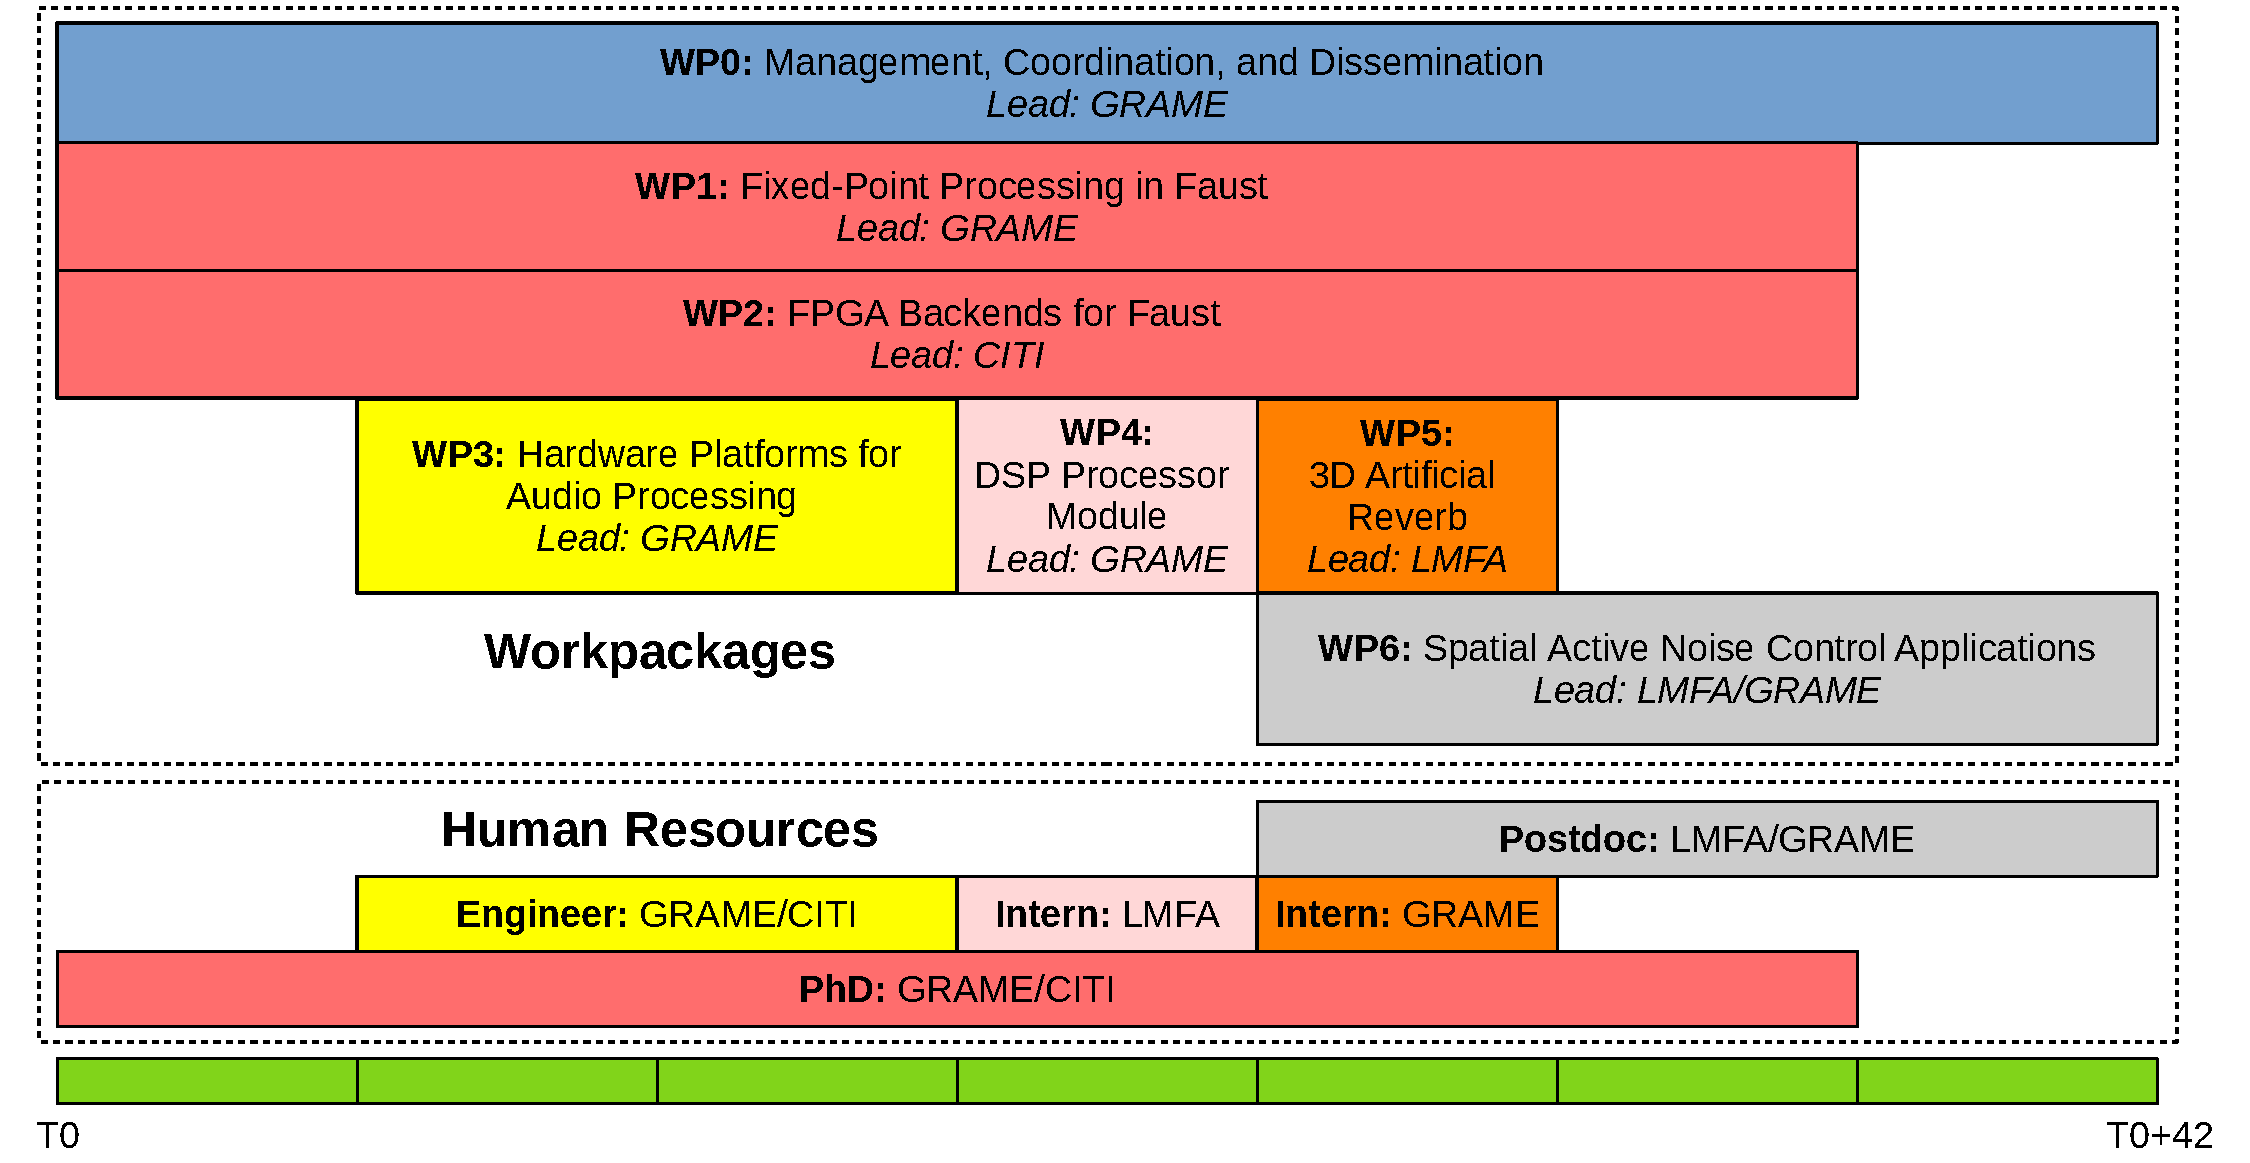
\includegraphics[width=15cm]{img/wp.pdf}
%   \caption{\PP{} project organization and planning. A more detailed Gannt Chart can be found in Fig.~\ref{fig:gannt} on p.~\pageref{fig:gannt}.}
%   \label{fig:overview}
% \end{figure}

% This section first describes the methodology (i.e., work packages) that will be used to implement \PP{}. Fig.~\ref{fig:overview} provides a coarse-grained overview of the work packages and human resources associated to them. A more detailed Gannt Chart can be found in Fig.~\ref{fig:gannt} on p.~\pageref{fig:gannt}. The second part of this section is about risk management.

% Remove the folloing line for FULL_PROPOSAL
This section first describes the methodology (i.e., work packages) that will be used to implement \PP{}. A detailed Gannt Chart can be found in Fig.~\ref{fig:gannt} on p.~\pageref{fig:gannt}. The second part of this section is about risk management.

\subsubsection{WP0 -- Management, Coordination, and Dissemination}
\label{subsubsec:wp0}

\begin{center}
\begin{tabular}{c | c c | c c c | c}
\textbf{WP0 Leader} & \textbf{Start} & \textbf{End} & \textbf{Grame} & \textbf{CITI} & \textbf{LMFA} & \textbf{Total}\\
\hline
Grame, Michon & M0 & M41 & 4 P.m. & 4 P.m. & 4 P.m. & 12 P.m.
\end{tabular}
\end{center}

\paragraph{T0.0 -- Project Management and Scientific Coordination}

\textit{T0.0 will start at M0 and end at M41. Total effort is 6 P.m: Grame 2, CITI 2, and LMFA 2.}

This task consists in: (1) Project management and planning (progress analysis and task coordination); (2) Consortium agreement, legal and intellectual property management; (3) Budget management; (4) Risk management (identification, assessment, and risk control) and potential project strategy updates; (5) Identification and resolution of potential conflicts; (6) Management of shared resources (e.g., web sites, wiki, code repositories, shared equipment); (7) Organization of internal meetings; (8) Monitoring of tasks deliverable, reports, cost statements, publications.

\paragraph{T0.1 -- Dissemination}

\textit{T0.1 will start at M0 and end at M41. Total effort is 6 P.m: Grame 2, CITI 2, and LMFA 2.}

\begin{itemize}
\setlength\itemsep{0em}
\item A website will present the project, the partners, the publications, and the tools developed as part of \PP{}.
\item There is a potential for multiple ``popular science'' publications on this project (i.e., actively modifying the acoustics of rehearsal room, developing ultra-low latency audio effects and synthesizers, reproduction of lost acoustic spaces: archeoacoustics, etc.). 
\item Workshops will be organized on the technology/tools developed in the framework of \PP{} in French institutions interested in these topics and at Stanford University (where R. Michon is one of the instructors of the \textit{CCRMA Summer Workshops Series}\footnote{\url{https://ccrma.stanford.edu/workshops}}).
\item One of Grame's Music Production Department's missions is to host artist residencies year-round. In that context, artist residencies will be organized at Grame to exploit/abuse the tools, systems, and technologies developed as part of \PP{}.
\item Another mission of Grame's Music Production Department is to organize concerts. Hence, we'll take advantage of Grame's experience and resources in this field to organize concerts leveraging the technology developed as part of \PP{}.
\item The technology developed as part of \PP{} will be demonstrated to the public through events at LMFA's listening room/studio where live and fixed-media performances will be carried out (see WP4). 
\item The results of the project will be published in scientific journals, proceedings of international conferences and seminars, etc.
\end{itemize}

\begin{center}
\begin{tabular}{c | c | c}
\textbf{Deliverable of WP0} & \textbf{Due Date} & \textbf{Leader}\\
\hline
\hline
\textbf{D0.0} -- Consortium Agreement & M7 & Grame\\
\hline
\textbf{D0.1} -- 1st Interim Management Report & M17 & Grame\\
\hline
\textbf{D0.2} -- 2nd Interim Management Report & M29 & Grame\\
\hline
\textbf{D0.3} -- Final Management Report & M41 & Grame
\end{tabular}
\end{center}

\subsubsection{WP1 -- Fixed-Point Processing in \F{}}
\label{subsubsec:wp1}

\begin{center}
\begin{tabular}{c | c c | c c c | c}
\textbf{WP1 Leader} & \textbf{Start} & \textbf{End} & \textbf{Grame} & \textbf{CITI} & \textbf{LMFA} & \textbf{Total}\\
\hline
(Grame, Letz) & M0 & M35 & 7 P.m. & 32 P.m. & 0 P.m. & 39 P.m.
\end{tabular}
\end{center}

\begin{figure}[ht]
  \begin{center}
    \begin{tabular}{cc}  \begin{boxedminipage}{9cm}
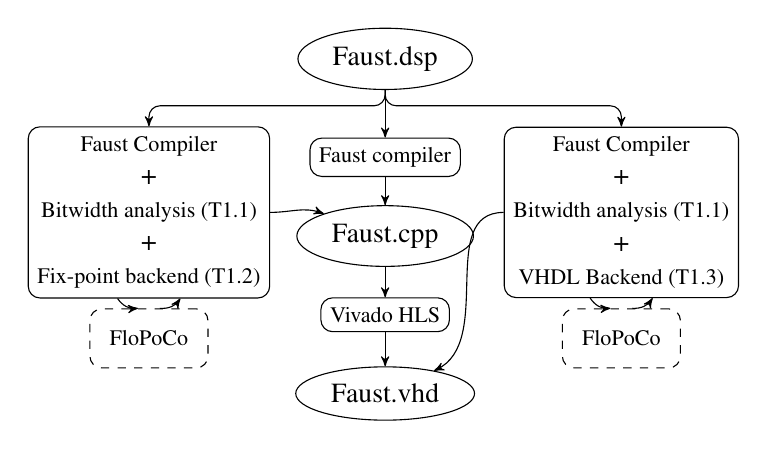
\begin{tikzpicture}[>=stealth']
	\node[ellipse, draw=black] (dsp) at (0,0){Faust.dsp};
	\node[rounded corners=0.15cm, draw=black, below of=dsp, yshift=-.25cm]
(fstCompile){\footnotesize Faust compiler};
	\node[rounded corners=0.15cm, draw=black, left of=fstCompile,align=center,xshift=-2cm, yshift=-.7cm]%
(fstCompileBitWidthCpp) {\footnotesize Faust Compiler\\+\\ \footnotesize Bitwidth  analysis (T1.1) \\+\\ \footnotesize Fix-point backend (T1.2)};
	\node[rounded corners=0.15cm, draw=black, right of=fstCompile,align=center,xshift=2cm, yshift=-.7cm]%
(fstCompileBitWidthHDL) {\footnotesize Faust Compiler\\+\\ \footnotesize Bitwidth  analysis (T1.1)\\+\\ \footnotesize VHDL Backend (T1.3) };

	\draw (dsp.south) ++(0, -.2) coordinate(junction);
	\draw [rounded corners, ->] (dsp.south) -- (junction) -| (fstCompileBitWidthCpp.north); 
	\draw [rounded corners, ->] (dsp.south) -- (junction) -|(fstCompileBitWidthHDL.north); 
	\draw[->] (dsp.south) -- (fstCompile);
	
	\node[draw=black, ellipse, below of=fstCompile] (cFstCpp) {Faust.cpp};
	\draw[->] (fstCompile.south) -- (cFstCpp.north);
	\node[draw=black, rounded corners=0.15cm, below of=cFstCpp](cVHLS){\footnotesize Vivado HLS};
	\draw[->] (cFstCpp) -- (cVHLS);
	\node[draw=black, ellipse, below of=cVHLS] (fstVHD){Faust.vhd};
	\draw[->] (cVHLS) -- (fstVHD);

	\node[dashed, minimum width=1.5cm, minimum height=.75cm, yshift=-.6cm, rounded corners=0.15cm, draw=black, below of=fstCompileBitWidthCpp]%
		(flopocoL) {\footnotesize FloPoCo};
	\draw[->] (fstCompileBitWidthCpp.250) [bend right] to (flopocoL.110);
	\draw[->] (flopocoL.70) [bend right] to (fstCompileBitWidthCpp.290);
	\draw[->] (fstCompileBitWidthCpp.east) [out=0, in=160] to (cFstCpp); 

	\node[dashed, minimum width=1.5cm, minimum height=.75cm,yshift=-.6cm, rounded corners=0.15cm, draw=black, below of=fstCompileBitWidthHDL]%
		(flopocoR) {\footnotesize FloPoCo};
	\draw[->] (fstCompileBitWidthHDL.250) [bend right] to (flopocoR.110);
	\draw[->] (flopocoR.70) [bend right] to (fstCompileBitWidthHDL.290);
	\draw[->] (fstCompileBitWidthHDL.west)  [out=180, in=25] to (fstVHD.25);

\end{tikzpicture}
\vspace{0.1cm}
\end{boxedminipage}
 & \begin{boxedminipage}{6cm}
  \begin{tikzpicture}[>=stealth']
	\node[ellipse, draw=black] (dsp) at (0,0){Faust.dsp};
	\node[rounded corners=0.15cm,align=center, draw=black, below of=dsp, yshift=-.25cm,text width=2.6cm]
        (fstCompile) {\footnotesize Faust Compiler\\ (from  WP1)};

	\draw[->] (dsp.south) -- (fstCompile);
	\node[draw=black, ellipse, below of=fstCompile] (cFstCpp) {Faust.cpp};
        \draw[->] (fstCompile.south) -- (cFstCpp.north);
        \node[draw=black, rounded corners=0.15cm, below of=cFstCpp](cVHLS){\footnotesize Vivado HLS};
  
    \node[ right of=dsp,align=center,xshift=2cm, yshift=-0.5cm] (bd) 
      {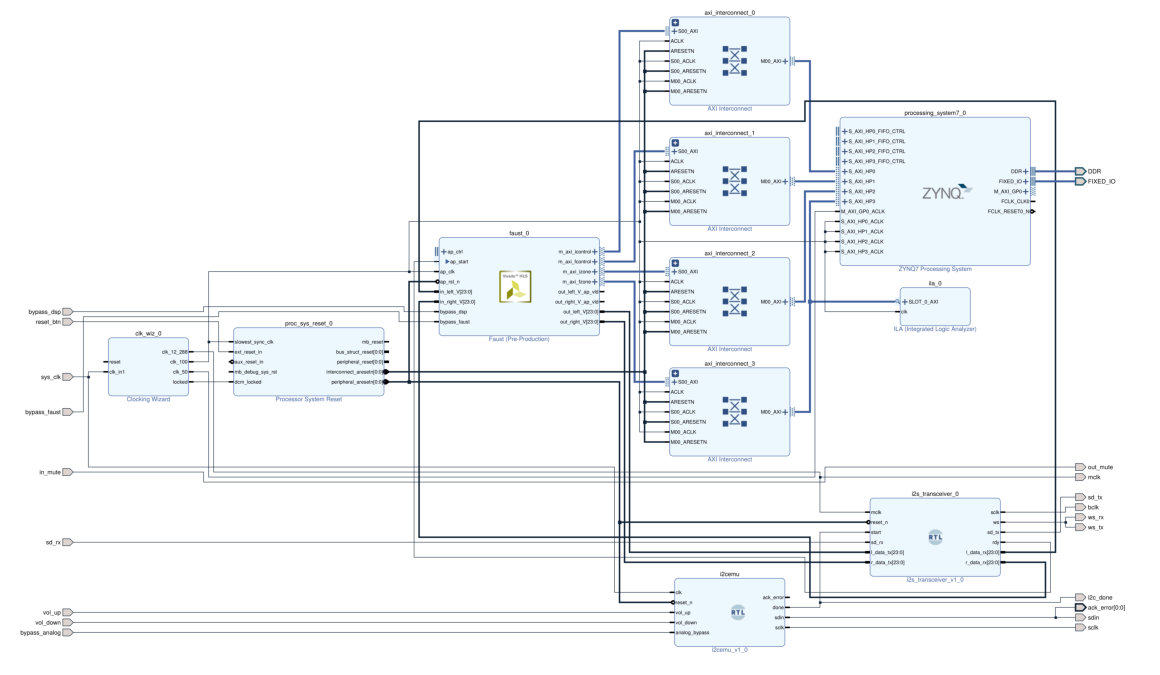
\includegraphics[width=2cm]{design_whole_zoom.pdf}};
    \node[ above of=bd,align=center,xshift=-0.5cm, yshift=-0.7cm] (blockdesign) {\scriptsize vivado block design};

    
	\draw[->] (cFstCpp) -- (cVHLS);
	\node[draw=black, ellipse, below of=cVHLS] (fstVHD){Faust.vhd};
	\draw[->] (cVHLS) -- (fstVHD);
	\node[draw=black, rounded corners=0.15cm, below of=bd, yshift=-0.2cm](vivado){\footnotesize Vivado};
        \draw[->] (bd.south)  to (vivado.north); 
	\draw[->] (fstVHD)  [out=25, in=185] to (bd.center);

	\node[minimum width=1.5cm, yshift=0cm,minimum height=0.75cm,fill=gray!20,draw=black, below of=vivado] (bitstream) {bistream.bit};
	\draw[->](vivado)--(bitstream);
            \node[ below of=bitstream,align=center,xshift=0cm, yshift=0cm] (zybo) 
    {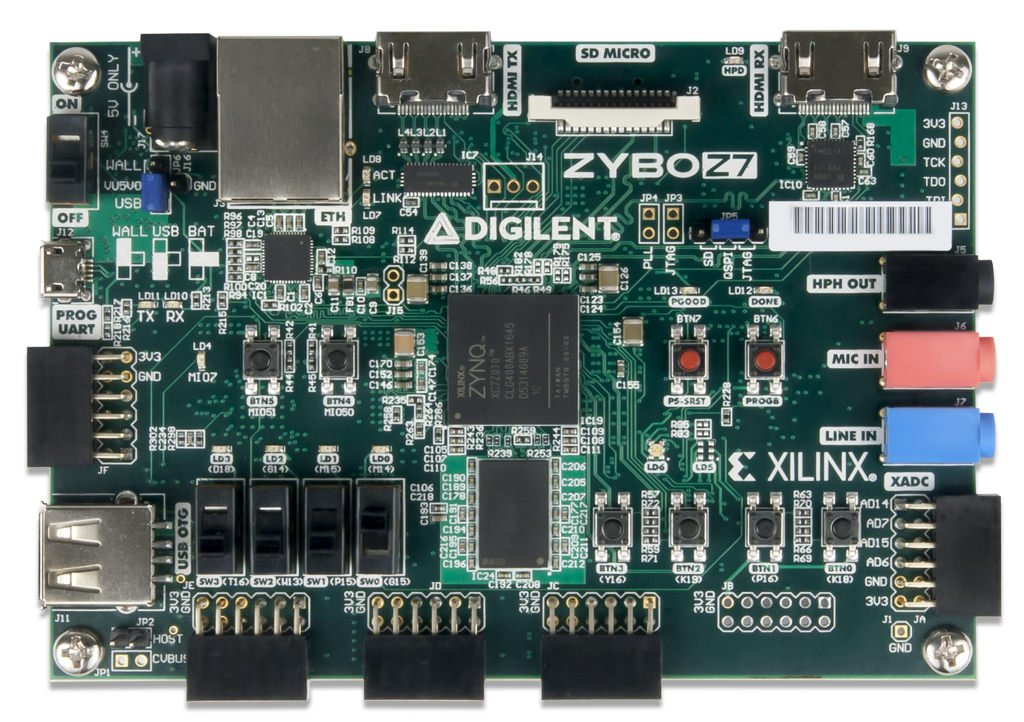
\includegraphics[width=1.5cm]{zybo.jpg}};
    \draw[->, line width=2, color=gray] (bitstream.south) [out=270, in=90] to (zybo.center); 
    \node[ below of=zybo,align=center, yshift=0.2cm] (zb) 
    {\scriptsize Zybo board};

\end{tikzpicture}
\end{boxedminipage}
 \\
      (a) & (b)
    \end{tabular}
  \end{center}
  \caption{(a) Different possible compilation flows for generating VHDL from a \F{} program studied in WP1. Round boxes are files (i.e., format), squared boxes are tools. Dashed boxes are tools outside the compilation flow used to tune the architecture. (b) The complete faust2fpga flow engineered in WP2}
  \label{fig:flows}
  \label{fig:synflow}

\end{figure}

Up to now, the \F{} compiler has only been producing floating-point C++ code since it mostly targets CPUs. This work package focuses on integrating in the \F{} compiler the required technologies to use fixed-point arithmetic in the generated code. The key idea is to use the arithmetic expertise of CITI-Lab ~\cite{volkova:hal-01561052} to infer the bitwidth for each variable in a \F{} program in order to ensure high sound quality in the most efficient way. This will be carried out in task T1.1. Once that is done, we will be able to produce fixed-point DSP C++ code, extending the current C++ \F{} backend to target HLS tools (leftmost path in Fig.~\ref{fig:flows}-(a)). Alternatively, we will directly generate VHDL using the existing FloPoCo VHDL backend (rightmost path in Fig.~\ref{fig:flows}-(a)).

The middle path in Fig.~\ref{fig:flows}-(a) is the easiest and currently only supported one: the \F{} compiler is ``tuned'' to output C++ code that fits into {\tt vivado\_hls} tools. Audio samples are coded on floats in that case. This flow will be studied in WP2 because many important optimizations are independent of the type chosen for the computation (i.e., memory access organization).

The left flow of Fig.~\ref{fig:flows}-(a) adds fixed-point optimization.  Here, the types used for computation are fixed-point of arbitrary width. First, an analysis of the \F{} data-flow graph should indicate what the required bit-width for each signal is, then the C++ code is generated accordingly and sent to {\tt vivado\_hls} using dedicated arithmetic operators. The type of analysis performed here is routinely performed in the {\tt FloPoCo} tool~\cite{flopoco}, and for some well identified sub-blocks such as IIR filters~\cite{volkova:hal-01561052} or trigonometric functions~\cite{DinIstSer2013-HEART-SinCos,DinIsto2015}, the bitwidth optimization code within FloPoCo can be used directly. This will be carried out in task T1.2.

Finally (right flow), for some \F{} program that are compute-bound, it might be interesting to think of a direct compiler from \F{} to VHDL. Indeed, the \F{} flow graph representation is close to a structural representation of the computations. The main difficulty here lies in the inference of memory accesses. For mundane tasks of VHDL generations, the FloPoCo VHDL backend \cite{flopoco} can be used. It also offers additional low-level arithmetic optimizations currently out of reach of HLS tools \cite{DinIstSer2013-FPL-BitHeap}. This will be studied in task T1.3.

\paragraph{T1.0 -- Survey and Bibliography of float2fixed Methodology}

\textit{T1.0 will start at M0 and end at M6. Total effort is 5 P.m.: Grame 1, CITI 4, and LMFA 0.}

This task will be responsible for choosing the strategies that will be explored for inferring fixed-point signal bitwidth in \F{} programs. This will imply a complete survey of existing techniques~\cite{float2fixed2,cairn,sentieysid,volkova:hal-01561052} and industrial tools (e.g., Matlab, Xilinx \cite{XilinxFloat2Fixed}, etc.). However we do not intend to develop a universal float-to-fix methodology as most of the existing ones work. Instead, we wish to exploit the domain knowledge available in the consortium. Some are trivial (e.g., inputs from ADCs and outputs to DACs are 16- to 24-bit fixed-point formats), some are more advanced (e.g., higher frequencies do not require the same resolution as lower ones, etc.). The role of this task will be to express constraints on the range and resolution of stream samples in a \F{} program, then define algorithms to propagate and solve these constraints until a fixed-point format can be associated to each variable. It will follow the {\em ``computing just right''} paradigm successfully exploited at CITI in other domains.

\paragraph{T1.1 -- Integration of Fixed-Point in Faust Compiler}

\textit{T1.1 will start at M3 and end at M18. Total effort is 13 P.m.: Grame 2, CITI 11, and LMFA 0.}

The methodology and algorithms discussed in the previous task should then be implemented in the \F{} compiler. This means selecting a fixed-point library and implementing possibly complex algorithms~\cite{volkova:hal-01561052} for choosing the bitwidth of each stream manipulated by \F{}. This task should finally deliver the first compilation of \F{} code to fixed-point C++ programs (Deliverable D1.0). We also expect this work to be usefull for other hardware targets, such as CPUs without floating-point unit.

\paragraph{T1.2 -- Generation of Fixed-Point C++ Code for HLS}

\textit{T1.2 will start at M6 and end at M35. Total effort is 6 P.m.: Grame 1, CITI 5, and LMFA 0.}

Interaction with the HLS tool ({\tt vivado\_hls}) has to be carefully studied: optimizations, in particular pipelining, provided by {\tt vivado\_hls} should not be blocked by the use of dedicated fixed-point operators. This task should optimize the faust2fpga design Flow delivered in T2.0: we except a complexity improvement of at least one order of magnitude for the generated designs.

\paragraph{T1.3 -- Generation of VHDL Directly from \F{}}

\textit{T1.3 will start at M12 and end at M35. Total effort is 15 P.m.: Grame 3, CITI 12, and LMFA 0.}

Another positive outcome of this task will be to make the  \PP{} results independent from Xilinx tools. However it is probably too ambitious to target {\em all} possible \F{} programs. We except to issue (D1.1) the first faust2VDHL tool.

This task will attempt to identify \F{} programs where direct VHDL compilation would be more efficient. While HLS tools are now very capable, there is a wide range of optimization opportunities that are currently out of their reach, for instance the possible fusion of a fixed-point sum of products in a single sum of weighted bits~\cite{fs97,DinIstSer2013-FPL-BitHeap}: this happens a lot in digital signal processing~\cite{volkova:hal-01561052}. 

\begin{center}
\begin{tabular}{p{12cm} | c | c}
\textbf{Deliverable of WP1} & \textbf{Due Date} & \textbf{Leader}\\
\hline
\hline
\textbf{D1.0} -- \F{} Compilation Towards Fixed-Point C++ Programs & M18 & Grame\\
\hline
\multicolumn{3}{p{16cm}}{This software deliverable will enable fixed-point designs to be compiled. Optimization of this tool-chain will be proceeded throughout the project.}\\
\hline
\hline
\textbf{D1.1} -- First faust2VDHL Direct Compilation Flow & M35 & Grame\\
\hline
\multicolumn{3}{p{16cm}}{This software module will allow to generate VHDL directly from \F{} without depending on Xilinx {\tt vivado\_hls}. It will most probably apply to a subset of \F{} programs to be defined.}\\
\end{tabular}
\end{center}

\subsubsection{WP2 -- FPGA Backends for \F{}}

\begin{center}
\begin{tabular}{c | c c | c c c | c}
\textbf{WP2 Leader} & \textbf{Start} & \textbf{End} & \textbf{Grame} & \textbf{CITI} & \textbf{LMFA} & \textbf{Total}\\
\hline
CITI, Risset & M0 & M35 & 5 P.m. & 20 P.m. & 0 P.m. & 25 P.m.
\end{tabular}
\end{center}

Obtaining VHDL from a \F{} program is not sufficient to {\em compile} \F{} programs to FPGAs. Indeed, the real design space exploration will take place during the {\em high-level synthesis} of the C++ code generated by \F{} compiler (using an existing HLS tool) and during the {\em block design} tuning. As mentioned earlier, we have chosen to use Xilinx hardware board and software tools ({\tt vivado\_hls} and {\tt vivado}). However, different types of boards can be targeted. In particular, a low cost board (e.g., Zybo,\footnote{\url{https://www.xilinx.com/products/boards-and-kits/1-4azfte.html}} the successor of Zedboard) and free webpack Xilinx software suite will be used for our compilation flow development. Conversely, a high performance FPGA (e.g., with Zynq UltrasScale\footnote{\url{https://store.digilentinc.com/genesys-zu-zynq-ultrascale-mpsoc-development-board/}}) and Vivado HL Design Editions will be used for the applications of WP3 and WP4, if needed.  

%% \begin{figure}[ht]
%%   \centerline{\begin{boxedminipage}{6cm}
  \begin{tikzpicture}[>=stealth']
	\node[ellipse, draw=black] (dsp) at (0,0){Faust.dsp};
	\node[rounded corners=0.15cm,align=center, draw=black, below of=dsp, yshift=-.25cm,text width=2.6cm]
        (fstCompile) {\footnotesize Faust Compiler\\ (from  WP1)};

	\draw[->] (dsp.south) -- (fstCompile);
	\node[draw=black, ellipse, below of=fstCompile] (cFstCpp) {Faust.cpp};
        \draw[->] (fstCompile.south) -- (cFstCpp.north);
        \node[draw=black, rounded corners=0.15cm, below of=cFstCpp](cVHLS){\footnotesize Vivado HLS};
  
    \node[ right of=dsp,align=center,xshift=2cm, yshift=-0.5cm] (bd) 
      {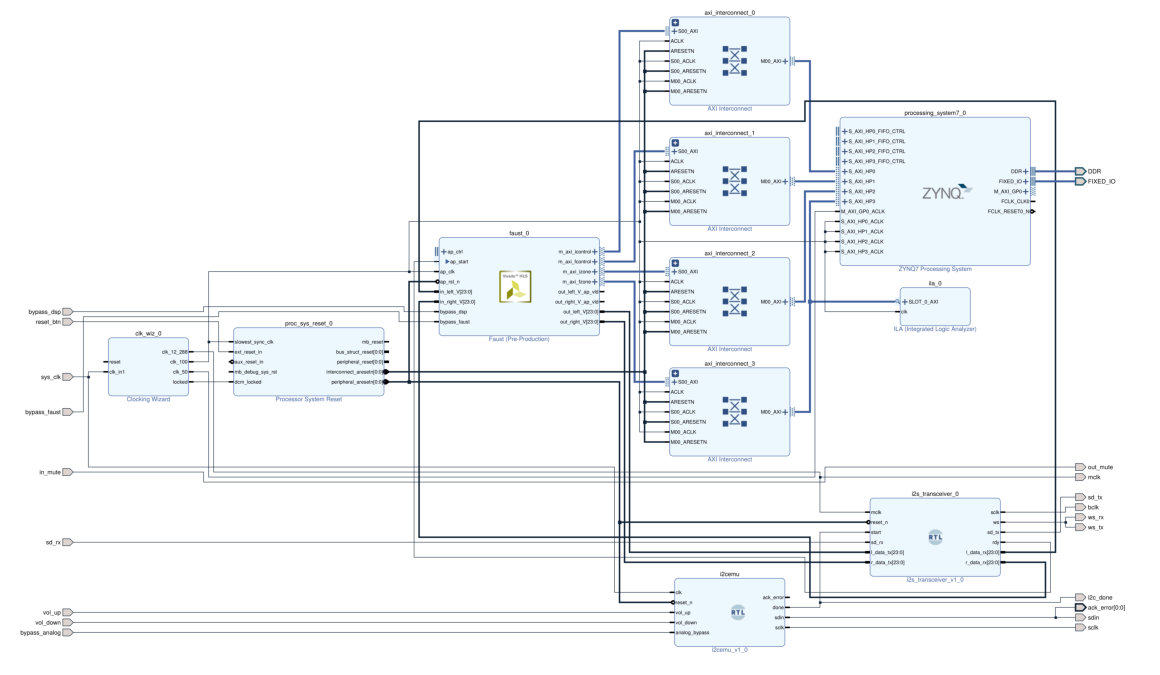
\includegraphics[width=2cm]{design_whole_zoom.pdf}};
    \node[ above of=bd,align=center,xshift=-0.5cm, yshift=-0.7cm] (blockdesign) {\scriptsize vivado block design};

    
	\draw[->] (cFstCpp) -- (cVHLS);
	\node[draw=black, ellipse, below of=cVHLS] (fstVHD){Faust.vhd};
	\draw[->] (cVHLS) -- (fstVHD);
	\node[draw=black, rounded corners=0.15cm, below of=bd, yshift=-0.2cm](vivado){\footnotesize Vivado};
        \draw[->] (bd.south)  to (vivado.north); 
	\draw[->] (fstVHD)  [out=25, in=185] to (bd.center);

	\node[minimum width=1.5cm, yshift=0cm,minimum height=0.75cm,fill=gray!20,draw=black, below of=vivado] (bitstream) {bistream.bit};
	\draw[->](vivado)--(bitstream);
            \node[ below of=bitstream,align=center,xshift=0cm, yshift=0cm] (zybo) 
    {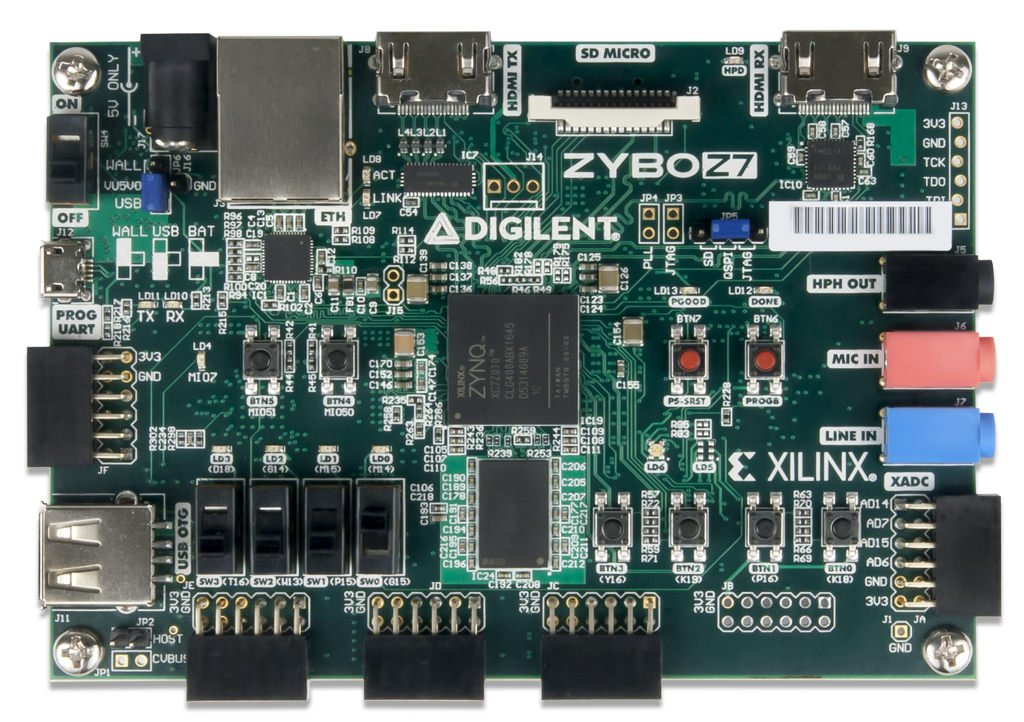
\includegraphics[width=1.5cm]{zybo.jpg}};
    \draw[->, line width=2, color=gray] (bitstream.south) [out=270, in=90] to (zybo.center); 
    \node[ below of=zybo,align=center, yshift=0.2cm] (zb) 
    {\scriptsize Zybo board};

\end{tikzpicture}
\end{boxedminipage}
}
%%   \caption{The complete faust2fpga flow engineered in WP2.}
%%   \label{fig:synflow}
%% \end{figure}

Fig.~\ref{fig:synflow}-(b) illustrates the generation of a {\em bitstream}, i.e., an FPGA binary file. In the so-called {\em block design}, the   \F{} IP generated from the VHDL code -- {\tt Faust.vhd} -- should be interfaced with:
\begin{enumerate}
\item The on-board audio codecs using I2C and I2S IPs.
\item The memory of the board (for storing samples when echo/delay is used)
\item The ARM processor that will interact with the \F{} IP.

\end{enumerate}

Important choices have to be made here which are usually referred to as {\em design space exploration}. These choices might depend on the target application and on the target board. They are related to the implementation of \F{} controllers, the memory architecture, and the schedule of the access to the different memories. These choices are the core of the different tasks of WP2.

\paragraph{T2.0 -- First faust2fpga Design Flow With Fixed-Point}
\textit{T2.0 will start at M3 and end at M12. Total effort is 5 P.m.: Grame 1, CITI 4, and LMFA 0.}

This task is responsible to produce the first automatic FPGA programming flow from \F{}. For that, many engineering issues have to be figured out: integration of fixed-point handling proposed in Task T1.1, interfacing with audio codec using I2S serial protocol and use of the processing subsystem (i.e., ARM processor) for initialization and control of the DSP treatment implemented. Following our recent proof of concept~\cite{risset2020}, we are confident in a rapid delivery of a functional design flow.

\paragraph{T2.1 -- Design Space Exploration for Memory Organization}
\textit{T2.1 will start at M9 and end at M24. Total effort is 10 P.m.: Grame 2, CITI 8, and LMFA 0.}

The compilation flow produced in the previous task (T2.0) will have to be optimized to produce more efficient results, either in terms of latency or in terms of computing power. There is a non-trivial design space exploration to perform in order to decide which audio samples should be stored on FPGA Block RAM and which should be stored in the external memory. External memory will imply slower treatment, but the treatment can be pipelined over successive samples (increasing latency, of course). This trade-off will be studied in order to produce a precise memory organization methodology depending on the constraint of the implemented DSP.

\paragraph{T2.2 -- Design Flow Adaptation for High Performance FPGA}
\textit{T2.2 will start at M18 and end at M35. Total effort is 5 P.m.: Grame 1, CITI 4, and LMFA 0.}

This task will provide the necessary adaptations of the compilation flow of Fig.~\ref{fig:synflow}-(b) to target the high-performance Zynq Ultrascale FPGA {\em Genesys ZU}. This target will be used for compute bound algorithms studied in WP5 (T5.1) and WP6 (T6.2). High computing power will need to optimize parallelization techniques used in the compilation flow (either by {\tt vivado\_hls} or by direct VHDL generation from \F{}). 

\paragraph{T2.3 -- Performance Study of the faust2fpga Compilation Flow}
\textit{T2.3 will start at M24 and end at M35. Total effort is 5 P.m.: Grame 1, CITI 4, and LMFA 0.}

An important outcome of the {\projectname} project is this new open-source compilation flow from \F{} to FPGA that will be useful in many contexts: for musicians, acoustic engineers or  vibration's mechanics engineers. In order to convince these people to use it, we have to prototype a large number of audio treatments (e.g., filters, reverb effects, etc.) and study the obtained performances -- in terms of latency and computing power again -- depending of the configuration chosen for the flow (as explained in  T2.1).

\begin{center}
\begin{tabular}{p{12cm} | c | c}
\textbf{Deliverable of WP2} & \textbf{Due Date} & \textbf{Leader}\\
\hline
\hline
\textbf{D2.0} -- First faust2fpga Design Flow With Fixed-Point & M12 & Citi\\
\hline
\multicolumn{3}{p{16cm}}{This software deliverable will enable fixed-point designs to be compiled on FPGA. It will constitute the basis of the compilation flow release occuring  throughout the project.}\\
\hline
\hline
\textbf{D2.1} -- faust2fpga Design Flow adapted for high performance FPGAFirst faust2VDHL Direct Compilation Flow & M35 & Citi\\
\hline
\multicolumn{3}{p{16cm}}{The software deliverable will consist in adapting the faust2fpga Design Flow to Ultrascale FPGA Genesys ZU for use in WP5 and WP6 }\\
\end{tabular}
\end{center}

\subsubsection{WP3 -- Hardware Platforms for Audio Processing}
\label{subsubsec:wp3}

\begin{center}
\begin{tabular}{c | c c | c c c | c}
\textbf{WP3 Leader} & \textbf{Start} & \textbf{End} & \textbf{Grame} & \textbf{CITI} & \textbf{LMFA} & \textbf{Total}\\
\hline
Grame, Michon & M6 & M17 & 14 P.m. & 1 P.m. & 1 P.m. & 16 P.m.
\end{tabular}
\end{center}

One of the main application of the technology that will be developed in WP1 \& WP2 is ultra-low latency audio processing. While the use of an FPGA solves this problem at the computational level, ultra-low latency can only be achieved if the audio ADC/DAC used by the system allows it. Since no FPGA board available on the market offers such feature, we'll have to make our own FPGA-based audio processor hosting ultra-low latency ADC/DAC. 

Two systems of this kind will be developed as part of WP3. \textbf{Module A} will take the shape of a circuit board connectable to the host FPGA board and providing a stereo audio input and output (2x2) as well as GPIOs. It will target the makers/music technology communities to prototype ultra-low latency/high performance electronic musical instruments, sound effect processors, etc. \textbf{Module B} will take the shape of a rackable module wrapped with some casing. Basic parameters will be configurable through a physical interface accessible on the front panel of the device (e.g., pots, buttons, etc.). It will target speaker and microphone arrays for active control of rooms acoustics and will therefore provide a greater number of inputs and outputs (32x32) but no GPIOs. Both modules will be programmable in \F{} through USB. Advanced software parameters linked to the \F{} program (i.e., \F{} DSP parameters) will be accessible through a web interface running a built-in server (see WP4).

While designing Module A will be relatively straight forward, handling 32x32 ultra-low latency channels on Module B will be more challenging and imply the implementation of additional custom hardware. Adding a I2C sensor ADC for GPIOs on Module A and for potentiometers and buttons on Module B should be straight forward.  

A research engineer will work at Grame on this project for one year under the guidance of Romain Michon and Pierre Lecomte.

\paragraph{T3.0 -- Multi-Channel Ulra-Low Latency Audio ADC/DAC}

\textit{T3.0 will start at M6 and end at M11. Total effort is 5 P.m.: Grame 5, CITI 0, and LMFA 0.}

This task will focus on designing a multi-channel (32x32) audio interface for ultra-low latency (below 100 $\mu s$). Audio PCM codecs will have to be selected and multiplexed to reach that goal. The deliverable for this task will be a PCB prototype ready-to-be-interfaced with the FPGA board that will be used as part of \PP{}.  

\paragraph{T3.1 -- FPGA-Based Audio Processors Design}

\textit{T3.1 will start at M9 and end at M15. Total effort is 9 P.m.: Grame 7, CITI 1, and LMFA 1.}

This task will center on designing Module A and B. Module A will just be a circuit board connectable/mountable on the host FPGA board. Module B should be rackable and easy to interface with our speaker and microphone array (see WP5). This will involve finalizing circuit design (e.g., balancing inputs and outputs for TRS connections, adding the front panel components I/Os, etc.), designing casings and front panel interfaces, and finally assembling working prototypes of the system.

\paragraph{T3.2 -- Final Testing, Production, and Fabrication}

\textit{T3.2 will start at M15 and end at M17. Total effort is 2 P.m: Grame 2, CITI 0, and LMFA 0.}

The final task of WP3 will focus on polishing the work carried out as part of T2.0 and T2.1 to release the final design of the two audio processors, finalize their datasheets and schematics, and potentially outsource their production if needed. The ability to access the DSP parameters of the \F{} program should ``come for free'' from the developments conducted in WP4.

\begin{center}
\begin{tabular}{p{12cm} | c | c}
\textbf{Deliverable of WP3} & \textbf{Due Date} & \textbf{Leader}\\
\hline
\hline
\textbf{D3.0} -- One 2x2 and One 32x32 Ultra-Low Latency FPGA-Based Audio Processor + Corresponding Report and Schematics & M17 & Grame\\
\hline
\multicolumn{3}{p{16cm}}{This hardware deliverable will consist of two ultra-low latency FPGA-based audio processors (one 2x2 channels and one 32x32 channels). It will come with a report describing the design of the system and the corresponding schematics.}\\
\hline
\hline
\textbf{D3.1} -- Report and Schematics on Module A and B & M17 & Grame\\
\hline
\multicolumn{3}{p{16cm}}{Report describing the design of the system and corresponding schematics.}\\
\end{tabular}
\end{center}

\subsubsection{WP4 -- DSP Processor Module}
\label{subsubsec:wp4}

\begin{center}
\begin{tabular}{c | c c | c c c | c}
\textbf{WP4 Leader} & \textbf{Start} & \textbf{End} & \textbf{Grame} & \textbf{CITI} & \textbf{LMFA} & \textbf{Total}\\
\hline
Grame, Michon & M18 & M23 & 8 P.m. & 1 P.m. & 3 P.m. & 12 P.m.
\end{tabular}
\end{center}

The stereo multi-channel ultra-low latency FPGA-based audio processor designed in WP3 (Module A) will be exploited in WP4 to turn into a flexible platform to implement sound effect processors/synthesizers, musical instruments, etc. This will involve the implementation of a software control interface including a GUI (Graphical User Interface) as well as MIDI and OSC support. Existing \F{} DSP libraries will be optimized for our platform and benchmarked in regard to other systems. Finally, demonstrators such as sound effect processors/synthesizers and musical instruments will be prototyped. This work will be carried by a masters-level intern hired as part of \PP{}.

\paragraph{T4.0 -- Software Control Infrastructure}

\textit{T4.0 will start at M18 and end at M20. Total effort is 4 P.m: Grame 3, CITI 1, and LMFA 0.}

FPGA development boards such as the Zybo\footnote{\url{https://www.xilinx.com/products/boards-and-kits/1-4azfte.html}} host an ARM CPU and run a full Linux distribution. The control portion of DSP algorithms with no ultra-low latency needs will run on the ARM processor (see WP2). T4.0 will focus on the development of a software interface running on the Linux system of the board to control the DSP portion running on its FPGA. This interface will include a web GUI (Graphical User Interface) running on an embedded web server accessible from outside of the board (e.g., WiFi, etc.) with a smart-device (e.g., smartphone, tablet, etc.) or a computer and will be controllable through MIDI and OSC. 

\paragraph{T4.1 -- Adapt \F{} DSP Algorithms}

\textit{T4.1 will start at M19 and end at M22. Total effort is 2 P.m: Grame 2, CITI 0, and LMFA 0.}

The \F{} DSP libraries \cite{Michon2017b} implement hundreds of algorithms for sound synthesis and processing. None of them was implemented with FPGA applications in mind, hence it is likely that a wide range of optimizations can be carried out to run them on the Module A DSP processor developed in WP3. This task will consist of reviewing and adapting existing algorithms from the \F{} DSP libraries for FPGA applications. Of course, new algorithms could be implemented as well and added to the libraries. This will also be a good time to run benchmarks to compare the performances of our system with traditional platforms.

\paragraph{T4.2 -- Musical Instruments and Sound Effect Processors}

\textit{T4.2 will start at M19 and end at M23. Total effort is 6 P.m: Grame 3, CITI 0, and LMFA 3.}

This task will focus on making demonstrators using the work from the two previous tasks. A programmable guitar pedal effect or a modular synthesizer based on Module A will be designed. Physical models of brass instruments based on Finite Difference in Time Domain algorithms will also be implemented \cite{Bilbao2009}.In order to demonstrate that an FPGA controller is a component particularly suited for the design of hybrid instruments, the soundboards of a guitar and a piano will be instrumented with sensors and actuators to apply active control algorithms with Module A. The playability of instruments will be validated with musicians. Controlling wind instruments is more challenging \cite{meurisse2015experimental}, but a demonstrator with a pipe will also be designed to test sound control algorithms before the  availability of Module B for WP6. 

\begin{center}
\begin{tabular}{p{12cm} | c | c}
\textbf{Deliverable of WP4} & \textbf{Due Date} & \textbf{Leader}\\
\hline
\hline
\textbf{D4.0} -- DSP Processor Module Software Control Infrastructure & M23 & Grame\\
\hline
\multicolumn{3}{p{16cm}}{This deliverable will consist in designing a software control infrastructure for our DSP processor module that will include: a web interface running on its own embedded web server and MIDI and OSC support.}\\
\hline
\hline
\textbf{D4.1} -- \F{} DSP Libraries Adapted to FPGA & M23 & Grame\\
\hline
\multicolumn{3}{p{16cm}}{This deliverable will consist in a collection of \F{} DSP libraries adapted for a use on our FPGA-based platform.}\\
\hline
\hline
\textbf{D4.2} -- Set of Sound Effect/Synthesizer Processors and Musical Instruments & M23 & Grame\\
\hline
\multicolumn{3}{p{16cm}}{This deliverable will consist in a set of demonstrators that will take the form of guitar pedal effects, modular synthesizer modules, musical instruments implementing active acoustic control, etc.}\\
\hline
\hline
\textbf{D4.3} -- Report on WP4 & M23 & Grame\\
\hline
\multicolumn{3}{p{16cm}}{This deliverable will consist of a report summarizing to work carried out in WP4. Its format will allow it to be transformed into a conference paper (e.g., SMC conference or NIME conference, etc.).}\\
\end{tabular}
\end{center}

\subsubsection{WP5 -- 3D Artificial Reverberation}
\label{subsubsec:wp5}

\begin{center}
\begin{tabular}{c | c c | c c c | c}
\textbf{WP5 Leader} & \textbf{Start} & \textbf{End} & \textbf{Grame} & \textbf{CITI} & \textbf{LMFA} & \textbf{Total}\\
\hline
LMFA, Lecomte & M18 & M29 & 1 P.m. & 1 P.m. & 11 P.m. & 13 P.m.
\end{tabular}
\end{center}

LMFA at École Centrale hosts a listening room with a 22.2 sound spatialization system with possibility for channel expansion. The goal of this work package is to use the 32x32 FPGA-based audio processor developed in WP3 to create a studio in LMFA's listening room where the reverberation of existing or modeled acoustical spaces will be experienced in three dimensions. We aim at organizing public events around this system towards the end of WP5 such as live performances and listening sessions. This work will be carried by a masters-level intern hired as part of \PP{}.

\paragraph{T5.0 -- Building the Studio}

\textit{T5.0 will start at M18 and end at M25. Total effort is 1 P.m: Grame 0, CITI 0, and LMFA 1.}

The goal of this task is to install the 32x32 FPGA-based audio processor developed in WP2 in the listening room of LMFA at École Centrale.
This will involve selecting gears, cabling, testing and calibrating the system in order to prepare and keep it up to date for the following tasks of WP5 and WP6. 

\paragraph{T5.1 -- Artificial Reverberation Algorithms}

\textit{T5.1 will start at M18 and end at M27. Total effort is 7 P.m: Grame 1, CITI 1, and LMFA 5.}

This task will leverage the work carried out during the first eighteen months of WP1 and WP2 to implement artificial reverberation algorithms in \F{} and run them in the setup implemented in T5.0. We'll target algorithms taking advantage of the inner properties of the FPGA (i.e., high-degree of parallelization). In particular, we believe that modal reverb \cite{Abel2019} -- which is hard/impossible to implement on standard computing platforms -- will find a very natural use-case with our system. This type of algorithm works by modeling the frequency response of a real or artificial acoustic space using a bank of second-order IIR filters which can be implemented with biquads. Filtering by the bank is an operation that can be highly parallelized and therefore adapted to the use of an FPGA. Moreover, since the parameters of each biquad can be modified on the fly, the resulting impulse response becomes parametric, which is not possible with linear convolutions. The use of modal reverb will for example allow to ``morph'' between several rooms. For instance, take the low frequency response of room A and high frequency response of room B, etc. A specific user interface will be developed to allow for the easy control of the reverberation parameters.
A possible extension of this technique could rely on spatial sound techniques. In fact, since IRs can be captured ``in 3D'' using an Ambisonics microphone, the convolution process can be carried out in 3D as well for the accurate rendering of spatial impression \cite{merimaa2005spatial}. Eventually, it will be possible to experience the reverberation of any existing space in 3D in LMFA's listening room or at home (through binaural/transaural technology) while keeping a high level of control on the system. 

\paragraph{T5.2 -- Landmarks Impulse Responses}

\textit{T5.2 will start at M24 and end at M27. Total effort is 2 P.m: Grame 0, CITI 0, and LMFA 2.}

The most exciting thing about WP5 is that we'll be able to experience the reverberation of any existing acoustic space in LMFA's listening room. The goal of this work package is to go on the field and make impulse response measurements of landmarks in the Lyon area to establish a catalog of reverberations that will be usable in LMFA's listening room. This database will then be a testimony of the acoustics of the Lyon environment at the time of the project and will be made freely available to the public. As the \PP{} project seeks to democratize the use of FPGAs to the greatest number of people, it will be possible to immerse oneself at home in a real or virtual place with the help of this database, using binaural/transaural technology.

\paragraph{T5.3 -- Public Events}

\textit{T5.3 will start at M27 and end at M29. Total effort is 3 P.m: Grame 0, CITI 0, and LMFA 3.}

This task will take place during the last month of WP5 and will be about opening LMFA's listening room to the public in order for it to experience the reverberation of various landmarks from the Lyon area or from around the world from a single standpoint. Recordings of performances could be played back through the system at specific hours. As the hardware system of WP3 is low-latency, the demonstrations will be interactive and not playback-only: the ambient sound in the studio will be captured with microphones and processed as well. Hence, the public will experience the reverberation of the room they have chosen. These demonstrations will pave the way for WP6. Indeed, the immersion effect can be greatly enhanced if the resulting sound field is precisely and physically controlled, which is what WP6 proposes.
 
\begin{center}
\begin{tabular}{p{12cm} | c | c}
\textbf{Deliverable of WP5} & \textbf{Due Date} & \textbf{Leader}\\
\hline
\hline
\textbf{D5.0} -- Listening Room/Studio For 3D Artificial Reverberation & M25 & LMFA\\
\hline
\multicolumn{3}{p{16cm}}{This deliverable will consist of preparing LMFA's listening room for 3D artificial reverberation applications using the system developed in WP3.}\\
\hline
\hline
\textbf{D5.1} -- Software Library in \F{} for 3D Artificial Reverberation & M27 & LMFA\\
\hline
\multicolumn{3}{p{16cm}}{This software deliverable will consist of a software library in \F{} for 3D artificial reverberation to be ran on the system implemented in D5.0.}\\
\hline
\hline
\textbf{D5.2} -- Database of 3D Impulse Responses & M27 & LMFA\\
\hline
\multicolumn{3}{p{16cm}}{This software deliverable will consist of a database of 3D impulse responses measured in landmarks of the Lyon area.}\\
\hline
\hline
\textbf{D5.3} -- Public Events Around the System Developed in WP3 & M29 & LMFA\\
\hline
\multicolumn{3}{p{16cm}}{A series of concerts and interactive listening sessions open to the public featuring the technology developed in WP5.}\\
\hline
\hline
\textbf{D5.4} -- Final Report on WP5 & M29 & LMFA\\
\hline
\multicolumn{3}{p{16cm}}{This repport will describe the work carried out as part of WP5 and should be ready to be turned into a conference paper (e.g., SMC conference).}\\
\end{tabular}
\end{center}

\subsubsection{WP6 -- Spatial Active Noise Control Applications}
\label{subsubsec:wp6}

\begin{center}
\begin{tabular}{c | c c | c c c | c}
\textbf{WP6 Leader} & \textbf{Start} & \textbf{End} & \textbf{Grame} & \textbf{CITI} & \textbf{LMFA} & \textbf{Total}\\
\hline
LMFA, Lecomte & M18 & M41 & 2 P.m. & 1 P.m. & 26 P.m. & 29 P.m.
\end{tabular}
\end{center}

In WP6, the LMFA listening room will be turned into a ``next generation rehearsal space'' for artists and musicians. By this, we mean a room whose acoustic field is physically controllable over a large region. For instance, musicians will be able to interact with the acoustics of the room where they will give their performance (e.g., a singer projecting his voice in a concert hall, musicians rehearsing in concert conditions but do not need to physically go to the concert venue, etc.).

In contrast with the techniques presented in \S\ref{sec:acr}, we wish to follow the approach of spatial active noise control here, whose recent algorithms are promising for controlling a continuous region of space \cite{lecomte2018cancellation,zhang2018active}. Thus, the minimization criteria will not be motivated by the listener's auditory system, but by a physical description of the target acoustic field. In contrast with WP5, an additional microphone array will be used here to continuously monitor the reconstructed sound field and feed the spatial active noise control algorithms to converge to the target. This physical approach is much more demanding in terms of sound field control, but we are convinced that it will bring greater realism and also open the way to many more applications: assistance in instrument making, archaeology, virtual reality, acoustic radiation from complex structures (e.g., aircraft engine, etc.). 

\begin{figure}[!htpb]
    \centering
    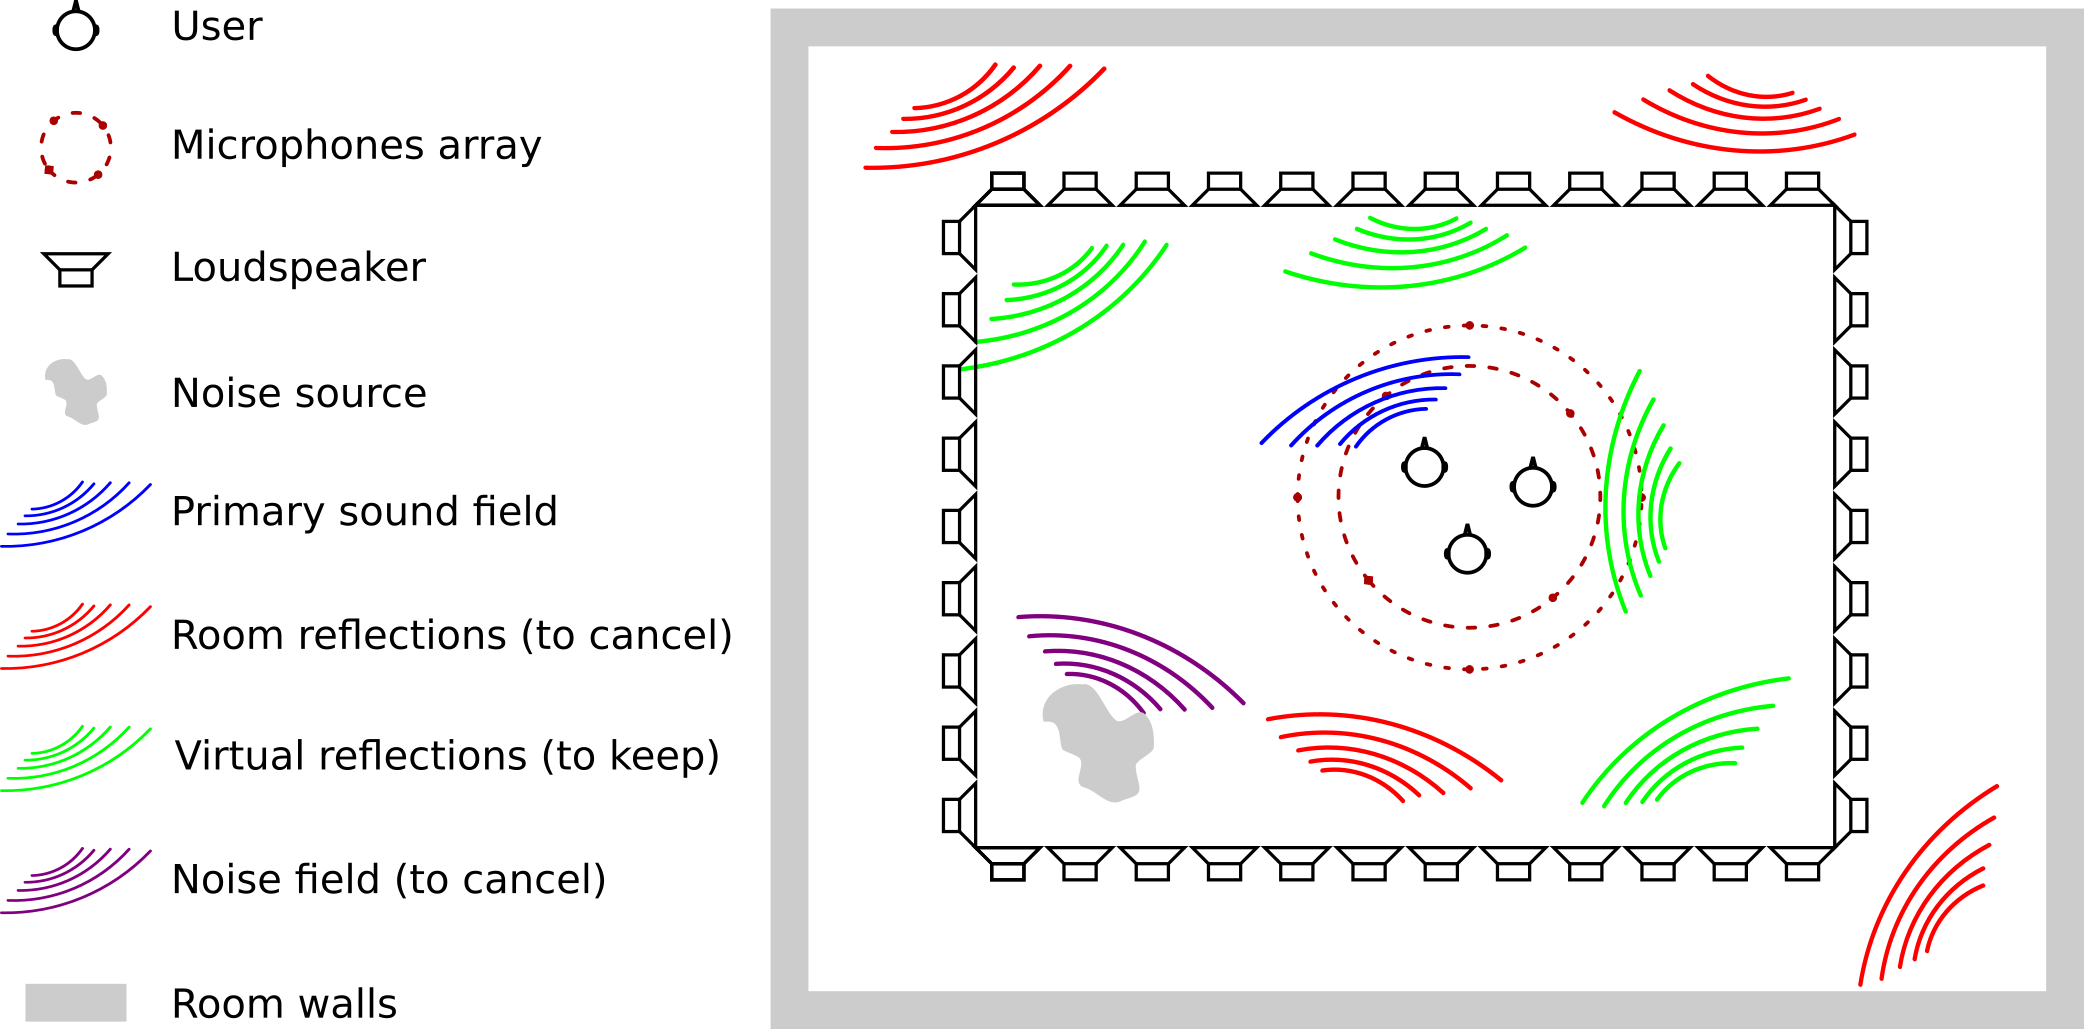
\includegraphics[width=13cm]{img/spatial_anc.png}
    \caption{A typical use-case of spatial active noise control: the primary sound field (in blue) is emitted by the artist inside the microphone array (user). The loudspeaker array is used as a secondary source to generate virtual reflections (green) and cancel any room reflections and noise fields (red, purple).}
    \label{fig:spatial_anc}
\end{figure}

A typical use case of what we are aiming to achieve in WP6 is shown in Fig.~\ref{fig:spatial_anc}. Artists stand in the room within a multi-radius open spherical microphone array. This array allows us to: (1) Decompose the total acoustic field on Spherical Harmonics basis  \cite{jin2014design} and capture its complexity including directivity \cite{pollow2009measuring}; (2) Separate the incoming and outgoing sound fields \cite{braikia2013evaluation}.

When artists produce a primary acoustic field (in blue), the microphone array picks up the radiated field and decomposes it on the spherical harmonics basis. This spatial information is sent to the 3D rendering system, which must generate the appropriate reflections (in green) to reproduce the reverberation of the desired location. Landmarks spatial impulse responses provided by T5.2 will be used here. However, parasitic reflections (in red) occur in the listening room which is not anechoic. In addition, possible noise sources may be present outside the microphone array (in purple). The challenge then is to be able to cancel the reflections and parasitic noise within the microphone volume, where the artists are located and keep the virtual reflections within this volume. To achieve this, a powerful spatial active control algorithm must be used as well as a powerful ultra-low-latency multi-channel system. The 32x32 FPGA-based audio processor developed in WP3 will be used to implement WP6. 

\paragraph{T6.0 -- Strategy and Algorithm Selection} 

\textit{T6.0 will start at M18 and end at M30. Total effort is 8 P.m: Grame 0, CITI 0, and LMFA 8.}

This first task consists of a literature review on classical, multi-channel active noise control \cite{elliott2000signal} and on recent approaches involving sound field decomposition \cite{lecomte2018cancellation,zhang2018active}. Based on this knowledge, the chosen strategy and development of a spatial active control algorithm will be carried out. Preliminary simulation results will be provided. Then, the algorithms will be adapted to target an implementation on the 32x32 system of WP3.

\paragraph{T6.1 -- Spatial Active Noise Control Over a Continuous Fixed Volume}


\textit{T6.1 will start at M30 and end at M36. Total effort is 11 P.m: Grame 1, CITI 1, and LMFA 9.}

The objective of this task is to validate experimentally, in the LMFA listening room, the spatial active control on a fixed volume.
The volume, bounded by a spherical microphone array, is fixed and cannot move. Indeed, to initialize the correction filters required by the spatial active noise control algorithm, an estimation of the acoustic transfer functions between the loudspeakers and the microphone array must be done \cite{lecomte2018cancellation}. As these functions depend on the location of the measurements, they should be remeasured if the correction volume were to move.

This task will be both experimental and theoretical. Indeed, the algorithms developed during the task T6.0 will most likely require some adaptations.

\paragraph{T6.2 -- Spatial Active Noise Control Over a Continuous Mobile Volume}

\textit{T6.2 will start at M36 and end at M41. Total effort is 10 P.m: Grame 1, CITI 0, and LMFA 9.}

In a second step, a more exploratory phase will propose to study the possibility of moving the controled volume. This requires an estimation in-situ of acoustic transfer functions. As this approach can be very demanding, a less constraining approach to the measurement volume can be taken, such as the transaural 3D restitution technique \cite{bharitkar2007immersive} (binaural restitution on a loudspeaker network with cancellation of crossed paths). Indeed, this technique requires to precisely reconstruct the pressure only at two points near the user's eardrums.


\begin{center}
\begin{tabular}{p{12cm} | c | c}
\textbf{Deliverable of WP6} & \textbf{Due Date} & \textbf{Leader}\\
\hline
\hline
\textbf{D6.0} -- Spatial Active Noise Control Working in Simulated Room & M30 & LMFA\\
\hline
\multicolumn{3}{p{16cm}}{This software deliverable will consist of spatial active noise control algorithms running on simulated rooms. }\\
\hline
\hline
\textbf{D6.1} -- Implementation of Spatial Active Field Control Algorithm and Validation Measurements Carried Out in LMFA Listening Room & M41 & LMFA\\
\hline
\multicolumn{3}{p{16cm}}{This deliverable will consist of an experimental set-up with spatial active noise control algorithms running on a fixed or mobile volume}\\
\hline
\hline
\textbf{D6.2} -- Final Report on WP6 & M41 & LMFA\\
\hline
\multicolumn{3}{p{16cm}}{This report will describe the work carried out as part of WP6 and should be ready to be turned into several journal and conference papers.}\\
\end{tabular}
\end{center}

\subsection{Risk Management}

\PP{} is deliberately ambitious, in particular in its scope that covers music, acoustics, DSP, FPGA programming, compilation, etc. However, this ambition is well within the frame of the complementary expertise of the project members (see \S\ref{subsec:consortium}) 

% FULL_PROPOSAL :
% \textbf{(1) Romain Michon} has expertise in audio embedded systems architecture, electronics, and DSP. In particular, his knowledge in circuit board development will be a great asset to the project especially in the context of WP3. \textbf{(2) Yann Orlarey} is the father of the \F{} programming language used at the heart of \PP{}. As such, he wrote the \F{} compiler and has all the required knowledge to modify/adapt it to the needs of \PP{}. \textbf{(3) Stéphane Letz} wrote a big part of the most recent \F{} backends (e.g., WebAssembly, \F{} interpreter, etc.), a knowledge which will be crucial in the context of WP1 and WP2. \textbf{(4) Tanguy Risset} has an extended experience in Compilation for embedded systems, FPGA programming and High Level Synthesis which are at the heart of WP1 and WP2. \textbf{(5) Florent de Dinechin} has a well-established expertise in non-standard hardware arithmetic design, in particular with this award-winning FloPoCo project which is central in WP1 and WP2. He also has a significant experience in small multiple-precision and mixed precision in the context of elementary function development and digital filters. \textbf{(6) Pierre Lecomte} has extended knowledge in spatial audio, in particular by developing the award-winning Ambitools project. These skills will be crucial in the context of WP5 and WP6. \textbf{(7) Marie-Annick Galland} is an expert in active control which is the central in WP6. She received the Plumey prize in 2005 for her contributions in that field. \textbf{(8) Sébastien Ollivier} is an expert in musical acoustics and musical instruments physical modelling.

The first risk is related to the feasibility of WP1 and WP2. Luckily, \PP{} builds upon the results of a previous project (SyFaLa \cite{risset2020}) where \F{}-generated objects can already be ran on FPGAs using Vivado HLS. The system is currently highly unoptimized so most of the work carried out as part of WP1 and WP2 will be related to improving this existing system to make it more efficient. In practice, this is linked to the main risk of \PP{} which is computational power. While we know that we'll be able to run a wide range of algorithms on our FPGA-based system, we also know that there will be limits to what can be done. These limits have yet to be determined.  

While designing the 2x2 audio DSP processor (Module A) of WP3 should be very straight forward, implementing Module B presents much greater challenges related to its extended number of audio channels (32x32). When having a system with 32 input and output channels at our disposal would be ideal, we could scale it down in case of an issue. In practice, this shouldn't be a problem thanks to use of ambisonics which will make our system very scalable.

WP4 presents very few risks and its implementation should be very straight forward.

WP5 will build upon the success of WP1, WP2, and WP3. Since the algorithms which will be used as part of WP5 (i.e., modal reverb) are quite expensive from a computational standpoint, this will be a good test case for the system implemented in WP1 and WP2. As we know how to implement these algorithms ``by hand'' (i.e., without going through \F{}) \cite{volkova:hal-01561052}, we have the guaranty that in the unlikely scenario where \F{}-generated objects would be too slow, we'd be able to make this system work. Similarly, using a smaller number of audio channels will not be a problem as well and will not compromise the success of WP5.


The topic of spatial active noise control is quite recent and few experimental results are available in the literature. This makes WP6 an ambitious work with a moderate risk that is commensurate with the ambition. However, the approaches towards which we are moving (decomposition of the acoustic field using spherical harmonics) are scalable. This makes it possible to limit the number of channels and the size of the control volume, without changing the theory. The realization of WP6 without the use of the system that will be implemented in the framework of the \PP{} remains possible, which limits the risk. The contribution of the 32x32 platform will only make WP6 more efficient and will offer new possibilities.

\section{Organization and Implementation}

\subsection{Scientific Coordinator and His Consortium}
\label{subsec:consortium}

Romain Michon is a researcher at GRAME-CNCM and a researcher and lecturer at the Center for Computer Research in Music and Acoustics at Stanford University (USA). His research focuses on embedded systems for real-time audio signal processing, Human Computer Interaction (HCI), New Interfaces for Musical Expression (NIME), physical modeling of musical instruments, digital fabrication techniques for music, and the \F{} programming language. 

Since 2018, one of his goal has been to make more accessible the programming of low-level embedded platforms such as microcontrollers \cite{Michon2019,Michon2020} for real-time audio signal processing applications through \F{}. These developments were used at the heart of the Amstramgrame project\footnote{\url{https://www.amstragrame.fr}} of which he is the main scientific coordinator. Amstramgrame aims at facilitating the teaching of maths and physics through the programming of embedded instruments called the Gramophones. The core idea of Amstramgrame is to make abstract scientific concepts more tangible through sound. Michon's knowledge in embedded systems will be very useful in the context of \PP{}. 

Romain Michon has been invested in the development of \F{} for the past ten years. In particular, he implemented various targets of the language (e.g., Android, microcontrollers, etc.) and he developed an environment for physical modeling of musical instruments based on \F{}.

As an active member of the music HCI community, he developed a wide range of interfaces and musical controllers such as Nuance \cite{Michon2016d} and the BladeAxe \cite{Michon2016}. This year, he's the paper chair of NIME (New Interfaces for Musical Expression)\footnote{\url{https://nime2020.bcu.ac.uk/}} which is the largest and most prestigious conference in this field.

Yann Orlarey is a researcher in Computer Music specializing in programming languages for music creation, sound synthesis, and audio signal processing. He is particularly interested in the creative and artistic use of functional programming, in particular, languages derived from $\lambda$-Calculus and Combinatory Logic. He is the designer, with his colleagues at Grame, of the \F{} programming language and its compiler. 

Stéphane Letz is a member of the Audio Working Group of the W3C, and a specialist in real-time audio architectures and music protocols. He is the designer of Jack2, the popular low latency audio server. He is also one of the main developer and maintainer of the \F{} compiler and ecosystem.

Romain Michon, Yann Orlarey, and Stéphane Letz all work at Grame which is a ``Centre National de Création Musicale'' (CNCM) organized in three departments: music production, transmission/mediation, and computer music research. Grame's research department has been leading the development of the \F{} programming language since its creation in 2004. It has expertise in computer science (compilation), audio DSP, digital lutherie, and HCI (Human Computer Interaction) in general. Thanks to the proximity of all three departments at Grame, research outcomes can easily find their way to professional musical productions and be shared with a general public through the organization of workshops and tight collaborations with the French ministry of education. Hence, the planning of concerts and outreach events around scientific culture leveraging the technology and research outcomes of \PP{} will be facilitated by Grame's general structure and strike force.

The two other academic partners of the project will be INSA-Lyon through the CITI laboratory (Center of Innovation in Telecommunications and Integration of Service) and Ecole-Centrale-Lyon through LMFA laboratory (Laboratoire de Mécanique des Fluides et d'Acoustique).

CITI lab will provide important skills about compilation, embedded systems, FPGA, high level synthesis and arithmetics operator implementations. Tanguy Risset (professor at INSA-Lyon) has been working for many years on HLS for FPGA (developer of the MMAlpha platform) before successively launching the creation of two Inria team-projects related to embedded systems (Compsys and Socrate). Florent de Dinechin (professor at INSA-Lyon) is one of the world specialist of arithmetic operators implementation on FPGA, he is also the creator of the FloPoCo tool that will be used in the project.  His expertise will be a unique opportunity to provide optimal FPGA designs.

LMFA (Laboratoire de Mécanique des Fluides et d'Acoustique) is a JRU (Joint Research Unit – UMR 5509). Its legal representatives are the Ecole Centrale de Lyon (ECL) and its linked third parties the Centre National de la Recherche Scientifique (CNRS), the Institut National des Sciences Appliquées de Lyon (INSA), and the Université Claude Bernard – Lyon I (UCBL). LMFA has leading expertise in acoustics, fluid mechanics, and active sound control. It hosts unique experimental facilities (i.e., anechoic rooms, wind tunnels, sound field synthesis rooms) which will be used for the experimental work of this proposal. Pierre Lecomte (associate professor at UCBL) has been working on sound field capture, control, and synthesis using loudspeakers and digital microphone arrays. He authored a plugin-suite (Ambitools) developed in \F{} for real-time sound field synthesis.\footnote{\url{https://www.sekisushai.net/ambitools}} Marie-Annick Galland (professor at École-Centrale Lyon) has been working on active noise/sound controls and supervised several PhD on the topic. Sébastien Ollivier (associate professor at UCBL) has been working on sound propagation and physical modeling of musical instruments.

\subsection{Means for Achieving the Objectives}

\begin{table}
\begin{center}
\begin{tabular}{c | r r r | r}
\textbf{Item of Expenditure} & \textbf{Grame} & \textbf{CITI} & \textbf{LMFA} & \textbf{Total}\\
\hline
\hline
\textbf{Staff on ANR} & 162 620 \euro{} & 110 988 \euro{} & 73 440 \euro{} & 347 048 \euro{} \\
\textbf{Staff NOT on ANR} & -- & 186 672 \euro{} & 89 120 \euro{} & 275 792 \euro{} \\
\textbf{Instruments and Material$^a$} & 15 300 \euro{} & 10 806 \euro{} & 20 000 \euro{} & 46 106 \euro{} \\
\textbf{Building and Ground} & -- & -- & -- & -- \\
\textbf{Service Delivery and Intellectual Property} & 8 400 \euro{} & 7 800 \euro{} & 3 000 \euro{} & 19 200 \euro{} \\
\textbf{Travel} & 20 000 \euro{} & 20 000 \euro{} & 20 000 \euro{} & 60 000 \euro{}\\
\textbf{Management and Structure}$^b$ & 84 369 \euro{} & 11 968 \euro{} &9 315 \euro{} & 105 652 \euro{} \\
\textbf{Full Cost} & 290 689 \euro{} & 348 234 \euro{} & 214 875 \euro{} & 853 798 \euro{} \\
\hline
\textbf{Total Requested} & 145 344 \euro{} & 161 562 \euro{} & 125 755 \euro{} & 432 661 \euro{} \\
\hline
\multicolumn{5}{p{14cm}}{a: Including scientific consumables. -- b: See the overhead costs sections for each partner below.}
\end{tabular}
\end{center}
\caption{Requested Means by Items of Expenditure and by Partners}
\label{tab:exp}
\end{table}


%%  TANG: décommenter cette partie pour faire les calculs exacts
%% \begin{table}
%% \begin{center}
%% \begin{spreadtab}{{tabular}{c|r r r |c}}
%%   \hline
%%   \textbf{@Item  of Expenditure} & \textbf{@Grame} & \textbf{@CITI} & \textbf{@LMFA} & \textbf{@Total}\\
%%   \hline
%%   \hline
%%   \textbf{@Staff on ANR} & 162620  & 110988  & 73440 &  sum(b2:d2)  \\
%%   \textbf{@Staff NOT on ANR} & 0 & 186672 & 89120  &  sum(b3:d3) \\
%%   \textbf{@Instruments and Material$^a$} & 15300 & 10806 & 19000 & sum(b4:d4)  \\
%%   \textbf{@Service Delivery and Intellectual Property} & 8400 & 7800 & 3000 & sum(b5:d5)  \\
%%   \textbf{@Travel} & 20000 & 20000 & 20000 & sum(b6:d6)\\
%%   \textbf{@Management and Structure} & 50*b2/100+7*sum(b4:b6)/100 & 8*(c2+sum(c4:c6))/100 & 8*(d2+sum(d4:d6))/100 & sum(b7:d7)  \\
%%   \textbf{@Full Cost} & 290689 & 349523 & 212266 & sum(b8:d8) \\
%%   \hline
%%   \textbf{@Total Requested} & 50*b8/100 & c2+sum(c4:c7) & d2+sum(d4:d7)  & b9+c9+d9 \\
%% \hline
%% \end{spreadtab}
%% \end{center}
%% \caption{Requested Means by Items of Expenditure and by Partners}
%% \label{tab:exp}
%% \end{table}

\begin{table}
\begin{center}
\begin{tabular}{c | c c c | c}
\textbf{Kind of Personnel} & \textbf{Grame} & \textbf{CITI} & \textbf{LMFA} & \textbf{Total}\\
\hline
\hline
\textbf{Permanent Staff on \PP{}} & 23 & 0 & 0 & 23\\
\textbf{Permanent Staff NOT on \PP{}$^a$} & 0 & 24 & 21 & 45\\
\textbf{Engineers} & 12 & 0 & 0 & 12\\
\textbf{Postdoc} & 0 & 0 & 18 & 18\\
\textbf{PhD Student} & 0 & 36 & 0 & 36\\
\textbf{Interns} & 6 & 0 & 6 & 12\\
\hline
\textbf{Total Effort} & 41 & 60 & 45 & 146\\
\hline
\multicolumn{5}{l}{a: Salary and other costs not charged on (i.e., not requested in) \PP{}.}
\end{tabular}
\end{center}
\caption{Overall Effort by Partners in P.m.}
\label{tab:effort}
\end{table}

\subsubsection{Partner 0: Grame}

{\secfont Staff Expenses}

\noindent
\begin{center}
\begin{tabular}{c | c | p{10cm}}
\textbf{Kind of Personnel} & \textbf{Effort} & \textbf{Justification}\\
\hline
\hline
Permanent Staff & 23 P.m. & Grame's permanent staff will be invested in all the work packages of the project\\
Engineer & 12 P.m. & An engineer will be recruited by Grame to carry out the work linked to WP3\\
Intern & 6 P.m. & An intern will be hired by Grame to carry out the work linked to WP4
\end{tabular}
\end{center}

{\secfont Instruments and Equipment Expenses}

\noindent
\begin{center}
\begin{tabular}{c | p{3cm} | r | p{10cm}}
\textbf{Scope} & \textbf{Item} & \textbf{Cost} & \textbf{Justification}\\
\hline
\hline
PW$^a$ & 2 Small FPGA Dev Boards & 600 \euro{} & Standard FPGA development boards to be used for R\&D by Grame's permanent staff throughout the project\\
\hline
PW & 1 Large/Powerful FPGA Deb Board & 1 200 \euro{} & Powerful FPGA development board to be used for specialized applications throughout the project\\
\hline
PW & 2 Laptops & 2 000 \euro{} & Laptops to be used by Grame's permanent staff throughout the project\\
\hline
PW & Small Array of Speakers & 6 000 \euro{} & Small speaker array (8 speakers) to prototype locally at Grame the systems implemented in WP3 and WP5\\
\hline
PW & Consumable Electronics & 1 000 \euro{} & E.g., sensors, ADC, etc. to be used throughout the project\\
\hline
WP3 & 1 Small FPGA Dev Board & 300 \euro{} & To be used for the 2x2 audio processor (Module A)\\
\hline
WP3 & 1 Large FPGA Dev Board & 1 200 \euro{} & To be used for the 32x32 audio processor (Module B)\\
\hline
WP3 & Electronic Parts & 3 000 \euro{} & For the audio processor modules\\
\hline
\hline
\multicolumn{2}{c}{\textbf{TOTAL}} 15 300 \euro{} \\
\hline
\multicolumn{4}{l}{a: Project Wide.}
\end{tabular}
\end{center}

{\secfont Service Delivery and Intellectual Property Expenses}

\noindent
\begin{center}
\begin{tabular}{c | p{3cm} | r | p{10cm}}
\textbf{Scope} & \textbf{Item} & \textbf{Cost} & \textbf{Justification}\\
\hline
\hline
PW$^a$ & Software Licences & 4 800 \euro{} & Software licenses for FPGA programming\\
\hline
WP3 & Casing Fabrication & 600 \euro{} & For the audio processor modules\\
\hline
WP3 & Circuit Board Printing \& Assembling & 3 000 \euro{} & For the audio processor modules\\
\hline
\hline
\multicolumn{2}{c}{\textbf{TOTAL}} 8 400 \euro{} \\
\hline
\multicolumn{4}{l}{a: Project Wide.}
\end{tabular}
\end{center}

{\secfont Travel Expenses}

\begin{center}
\begin{tabular}{c | r | r}
\textbf{Item} & \textbf{Unitary Cost} & \textbf{Total} \\
\hline
\hline
2 Journal Papers & 1 000 \euro{} & 2 000 \euro{}\\
\hline
6 International Conference Trips & 3000 \euro{} & 18 000 \euro{}\\
\hline
\hline
\multicolumn{2}{c}{\textbf{TOTAL}} 20 000 \euro{} \\
\hline
\end{tabular}
\end{center}

{\secfont Overhead Costs}

\noindent
Overhead costs at Grame consists in 50\% for staff expenses ($162,620\times0.5 = 81,310$ \euro{}) and 7\% for other expenses ($43,700\times0.07 = 3,059$ \euro{}) which corresponds to a total of 84,369 \euro{} (see Table~\ref{tab:exp}).

\subsubsection{Partner 1: CITI}

{\secfont Staff Expenses}

\noindent
\begin{center}
\begin{tabular}{c | c | p{10cm}}
\textbf{Kind of Personnel} & \textbf{Effort} & \textbf{Justification}\\
\hline
\hline
Permanent Staff & 24 P.m. & CITI's permanent staff will be invested in all the work packages of the project\\
PhD Student & 36 P.m. & A PhD student will be recruited by CITI to work on WP1 and WP2
\end{tabular}
\end{center}

{\secfont Instruments and Equipment Expenses}


\noindent
\begin{center}
\begin{tabular}{c | p{3cm} | r | p{10cm}}
\textbf{Scope} & \textbf{Item} & \textbf{Cost} & \textbf{Justification}\\
\hline
\hline
PW$^a$ & 2 Small FPGA Dev Boards & 600 \euro{} & Standard FPGA development boards to be used for CITI permanent staff throughout the project\\
\hline
WP2 & 1 Large/Powerful FPGA Deb Board & 1 200 \euro{} & Powerful FPGA development board for adapting faust2fpga workflow by PhD\\
\hline
WP2 & 1 Large/Powerful FPGA Deb Board & 1 200 \euro{} & Powerful FPGA development board for adapting faust2fpga workflow by PhD\\
\hline
PW & 3 Laptops & 6 000 \euro{} & one Laptop fot the PhD, one laptop for each permanent member\\
\hline
PW & Consumable Electronics & 3 000 \euro{} & E.g., sensors, ADC, etc. to be used throughout the project\\
\hline
\hline
\multicolumn{2}{c}{\textbf{TOTAL}} 10 806 \euro{} \\
\hline
\multicolumn{4}{l}{a: Project Wide.}
\end{tabular}
\end{center}

{\secfont Service Delivery and Intellectual Property Expenses}

\noindent
\begin{center}
\begin{tabular}{c | p{3cm} | r | p{10cm}}
\textbf{Scope} & \textbf{Item} & \textbf{Cost} & \textbf{Justification}\\
\hline
\hline
PW$^a$ & Software Licences & 4 800 \euro{} & Software licenses for FPGA programming\\
\hline
WP2 & Circuit Board Printing \& Assembling & 3 000 \euro{} & For the audio processor modules\\
\hline
\hline
\multicolumn{2}{c}{\textbf{TOTAL}} 7 800 \euro{} \\
\hline
\multicolumn{4}{l}{a: Project Wide.}
\end{tabular}
\end{center}

{\secfont Travel Expenses}

\begin{center}
\begin{tabular}{c | r | r}
\textbf{Item} & \textbf{Unitary Cost} & \textbf{Total} \\
\hline
\hline
2 Journal Papers & 1 000 \euro{} & 2 000 \euro{}\\
\hline
6 International Conference Trips & 3000 \euro{} & 18 000 \euro{}\\
\hline
\hline
\multicolumn{2}{c}{\textbf{TOTAL}} 20 000 \euro{} \\
\hline
\end{tabular}
\end{center}

{\secfont Overhead Costs}

\noindent
Overhead costs at INSA-Lyon consists in 8\% of the requested amount: $149,594 \times 0.08 = 11,968$ \euro{} (see Table~\ref{tab:exp}).

\subsubsection{Partner 2: LMFA}

{\secfont Staff Expenses}

\noindent
\begin{center}
\begin{tabular}{c | c | p{10cm}}
\textbf{Kind of Personnel} & \textbf{Effort} & \textbf{Justification}\\
\hline
\hline
Permanent Staff & 21 P.m. & LMFA's permanent staff will be invested in all the work packages of the project\\
Postdoc & 18 P.m. & A postdoc will be recruited by LMFA to work on WP6\\
Intern & 6 P.m. & An intern will be recruited by LMFA to work on WP5
\end{tabular}
\end{center}

{\secfont Instruments and Equipment Expenses}
\noindent
\begin{center}
%\begin{tabular}{c | p{3cm} | c | p{10cm}}
\begin{tabular}{p{1.6cm} | p{5.5cm} | c | p{9cm}}
\textbf{Scope} & \textbf{Item} & \textbf{Cost} & \textbf{Justification}\\
\hline
\hline
WP4	& An acoustic guitar, vibration actuators \& sensors, microphones, loudspeakers, amplifier, 2x48V supply, cables, mechanical parts & 2000 & To built active control demonstrators: a hybrid guitar, a piano soundboard control setup, a setup to test acoustic active control of a pipe  \\	
\hline
WP5-WP6	&  Loudspeakers &	3200	& Loudspeakers to complement or enhance the LMFA listening room \\
\hline 
WP5	& 5x Spherical Microphone Arrays &	6000 & 3D impulses responses capture and sound field analysis \\
\hline 
WP5	& 5x Proximity Microphones & 500 &	Microphone for capturing ``dry''
signals on users for demonstrations in the LMFA listening room \\
\hline 
WP5-WP6	& 2x 12 Channels Amplifier & 1000 &	Amplifier for complementary loudspeakers \\
\hline 
WP6	& 2x Multichannel DSP Boards & 2000	& Real-time DSP boards for the preliminary development of active control algorithms \\
\hline 
WP6	& 500x Digital MEMS Microphones	& 500 & Microphones for the microphone array used in WP6 \\
\hline 
WP5-WP6	& 2x Powerful Desktop/Laptops &	4000 &	Computers for the intern and post-doc \\
\hline 
WP5-WP6	& Cables, loudspeaker mounts, spare parts & 800	& Miscellaneous material for the assembly, wiring of the installations	\\
\hline
\hline
\multicolumn{2}{c}{\textbf{TOTAL}} 20 000 \euro{} \\
\hline
\multicolumn{4}{l}{a: Project Wide.}
\end{tabular}
\end{center}		

{\secfont Service Delivery and Intellectual Property Expenses}

\noindent
\begin{center}
\begin{tabular}{c | p{3cm} | r | p{10cm}}
\textbf{Scope} & \textbf{Item} & \textbf{Cost} & \textbf{Justification}\\
\hline
\hline
WP5-WP6 & Microphone arrays mounts structure &	3000 & Construction of a structure for a double-layer microphone array \\
\hline
\hline
\multicolumn{2}{c}{\textbf{TOTAL}} 3 000 \euro{} \\
\hline
\end{tabular}
\end{center}

{\secfont Travel Expenses}

\begin{center}
\begin{tabular}{c | r | r}
\textbf{Item} & \textbf{Unitary Cost} & \textbf{Total} \\
\hline
\hline
2 Journal Papers & 1 000 \euro{} & 2 000 \euro{}\\
\hline
6 International Conference Trips & 3000 \euro{} & 18 000 \euro{}\\
\hline
\hline
\multicolumn{2}{c}{\textbf{TOTAL}} 20 000 \euro{} \\
\hline
\end{tabular}
\end{center}

{\secfont Overhead Costs}

\noindent
Overhead costs at Centrale Lyon consists in 8\% of the requested amount: $115,440 \times 0.08 = 9.235$ \euro{} (see Table~\ref{tab:exp}).

\section{Project Impact and Benefits}

Audio DSP is used everywhere is nowadays life (e.g., smartphones, TVs, cars, tablets, computers, musical instruments, speakers, etc.). Computational power and low-latency are probably the most important technical factors when it comes to these types of systems. FPGAs can help take this field to a new level. This is only possible if this type of platform is easily accessible to non-FPGA engineers. We believe that \PP{} has the potential to revolutionize the field of real-time audio DSP in the same way than Arduinos disrupted the world of prototyping and engineering. Possibilities unveiled by these developments will impact a wide range of fields and could lead to plethora of technological and industrial applications to design concert halls of a new kind, suppress noise in a car's passenger compartment, diminish vibrations in airplane jet engines, improve existing digital musical instrument technologies, etc. \PP{} will also give birth to many scientific publications in all these fields.

\subsection{Expected Impact on the Music Technology and Makers Communities}

Just like the BELA \cite{mcpherson2015} brought low-latency to the music technology and makers communities for real-time audio DSP applications a couple of years ago, we want to make ultra-low-latency a reality for everyone! FPGA platforms are currently out of reach to these communities. One of the main ambition of \PP{} is to facilitate their programming using a high-level DSL (i.e., \F{}) in order for engineers, musicians, and makers to seize this technology and place it at the heart of their work. This will only be possible if we make open source developments a core element of \PP{} by targeting open source hardware as much as possible and by completely opening the software tools which will be implemented as part of this project. The Module A described in WP3 will target this type of applications by providing a platform for prototyping digital musical instruments, art installations, audio effect processors, etc. We also believe that it could easily find its way in start-up projects and open the door to a wide range of new developments in the music technology industry -- a market whose worldwide sales exceed \euro{}15 billion.

\subsection{Expected Impact on the Audio DSP Community}

The computational and ultra-low latency performances as well as the accessibility provided by the platform that will be developed as part of \PP{} will open the door to new research avenues for the audio DSP research community. On the computational plan, the high level of parallelization and modular architecture of FPGAs will provide new opportunities to run specific DSP algorithms in real-time. In particular, physical models of musical instruments using the Finite Difference Scheme Method \cite{Bilbao2009} could greatly benefit from this type of developments. Similarly, new types of artificial reverberation algorithms could be explored/implemented as this is already done as part of WP5. Ultra-low audio latency will make possible all sorts of research developments around active acoustic control of musical instruments \cite{meurisse2015experimental} and of rooms \cite{Zhang2018}. Similarly, research around audio spatialization and sound field rendering could be pushed forward by our developments. All these research fields are craving for an easily programmable ultra-low latency multi-channel audio processing system that we plan to develop as part of \PP{} (Module B -- see WP4). In particular, Stanford's CCRMA which is one of the world's leader in the field audio spatialization is extremely interested in such platform to use it to implement new generations of Wave Field Synthesis (WFS) systems, etc. 

All the research fields mentioned in this section are among the ``hotest'' in audio DSP nowadays which is why truly bieleve that our developments will be used by a lot of people.

\subsection{Expected Impact on the Active Control Community}

As mentioned in WP6, FPGA-based solutions for active control applications are the most suitable. The accessibility of this type of systems that will be provided as part of \PP{} will likely have a significant impact on the active control community. 

For instance, FPGAs could be easily used in the context of single-channel controllers: 
a theme already developed for active headsets \cite{benois2017fully}, for example. Ultra-low-latency allows for a fully digital feedback control to be implemented in this case. More generally, feedback control which was previously limited to small, non-modular spaces can be extended to a variety of situations, given the flexibility and adaptability of digital filters. 
Another extension could be the implementation of multichannel controllers. Experiments have already been performed for the design of multichannel feedforward FPGA controllers with the development of architectures adapted from the FXLMS reference algorithm \cite{shi2019practical}. This could lead the way to real/practical scale applications outside of the lab. 
In recent advances, some algorithms provide continuous noise control over large areas of space, (i.e., ``spatial noise control'')~\cite{lecomte2018cancellation,zhang2018active}.

\subsection{Expected Impact on the FPGA Community}

High Level Synthesis is a technology that enables the high-level programming of FPGAs. However, although this technology is quite mature, it is not really used by non-specialist because of the lack of high-level tools such as the one that will result from {\projectname}. As mentioned before, the HLS tools proposed earlier~\cite{pico,catapultC,gaut} start from a programming language (C, C++, or Python) which is {\em instrumented} using pragmas, making them quite hard to use for non-specialists. Our project will reveal that the use of domain specific languages, such as \F{} in our case, opens the doors to new generation FPGA compilers.

We believe that the result of {\projectname} are likely to have an important impact on FPGA research community as it will propose innovative compilation techniques to provide better FPGA compilers.

\subsection{Other Industrial Applications}

Beside the aforementioned applications in the music and makers/prototyping industries, we believe that the work carried out as part of \PP{} will find its way in the fields of automotive, acoustics, etc. We think that the ultra-low latency audio processor modules (see WP4) developed as part of \PP{} have an important role to play in that context by providing extended computational power for noise cancellation algorithms and lower latency performances than any other available system. Similarly, a few companies have been trying to develop systems for the active control of room acoustics. Meyer Sound Constellation System\footnote{\url{https://meyersound.com/product/constellation/}} is a good example of that. We believe that the platform developed as part of \PP{} has the potential to take this type of system to the next level. 

Industrial developments of active noise control systems have so far been limited either to small spaces (active headsets, low-frequency ducts for aeraulic systems) or to noises of a particular nature (e.g., periodic noise from propeller aircraft, land vehicle engines, etc.). 
FPGAs based solutions, which offer low-latency and high computational capabilities, will enable the extension of controlled volumes, and possibility of moving it. For instance in the automotive sectors with the reduction of road noise inside the passenger compartment \cite{jung2019local}.

Another application would be the active treatment of boundary conditions with the realisation of ``smart surfaces'' for absorption \cite{mazeaud2007multichannel,betgen2011new}, or vibro-acoustic isolation \cite{melon2012one,hu2012acoustic,zielinski2012fully}: Active material developments are based on multi-channel control systems combining global control and decentralised feedback systems. The use of FPGAs would enable them to be applied on a large scale, in buildings and also in transport systems (aircraft, turbojet nacelles). The LMFA is developing both the experimental means (MATISSE and CAIMAN test benches, ECL-B3 test bench from Equipex PHARE), and the numerical codes of acoustic propagation \cite{deng2019comparison,troian2017broadband}, within the framework of a strong partnership with Safran Aircraft Engines (ANR ADOPSYS and ARENA industrial chairs). The development of a high-level compiler dedicated to Acoustic Digital Signal processing on FPGA is therefore in high demand by many acoustic researcher for numerous industrial applications.

\subsection{Expected Impact Towards the Public}

The extremely applied type of research that will be carried out as part of \PP{} has countless of high-level and easily approachable applications which are all very tangible. In that context, we plan to organize a series of events (see WP0) demonstrating and promoting our technology. In particular, concerts and listening sessions open to the public at LMFA's listening room will allow the audience to experience the acoustics of various landmarks from the Lyon area within the same room. We will prototype a concept of ``rehearsing studio of the future'' where musicians can come and play in a space whose acoustic can be modified on demand. We will leverage Grame's experience to organize artist residencies around this system. We also plan to open this studio to local musical professional music institutions (e.g., opera, conservatoire, etc.). We also hope to be able to organize concerts taking advantage of these developments. For example, a concept we'd like to explore would be to have an immersive opera where the acoustic of the concert hall evolves in function of the scenes.

\PP{}'s research outcomes also have a lot of applications towards digital lutherie/musical instrument making, guitar pedal effect design, modular synthesizers, etc. which are all very approachable by the general public. Grame organizes events yearround (e.g., concerts, exhibitions, etc.) and we plan to showcase the instruments that will be developed as part of \PP{} in this context.


\begin{sidewaysfigure}[ht]
  \renewcommand\sfdefault{phv}
\renewcommand\mddefault{mc}
\renewcommand\bfdefault{bc}
\sffamily
\begin{ganttchart}[
    canvas/.append style={fill=none, draw=black!20, line width=1pt},
    x unit=0.4cm,
    y unit chart=0.46cm,
    hgrid style/.style={draw=black!20, line width=1pt},
    vgrid={*1{draw=black!20, line width=1pt}},
    title/.style={draw=none, fill=none},
    title label font=\bfseries\footnotesize,
    title label node/.append style={below=7pt},
    include title in canvas=false,
    bar label font=\mdseries\small\color{black!70},
    bar label node/.append style={left=.2cm},
    bar/.append style={draw=none, fill=black!63},
    bar incomplete/.append style={fill=barblue},
    bar progress label font=\mdseries\footnotesize\color{black!70},
    group incomplete/.append style={fill=groupblue},
    group left shift=0,
    group right shift=0,
    group height=.5,
    group peaks tip position=0,
    group label node/.append style={left=.2cm},
    group progress label font=\bfseries\small,
    milestone label font=\mdseries\small\color{black!70},
    milestone label node/.append style={left=.2cm},
    milestone inline label node/.append style={left=2mm}
  ]{0}{41}
  \gantttitle[
    title label node/.append style={below left=7pt and -3pt}
  ]{MONTHS:\quad0}{1}
  \gantttitlelist{1,...,41}{1} \\
  %%%%%%%%%%
  \ganttgroup[]{Management, Coordination, and Dissemination -- WP0}{0}{41} \\
  \ganttbar[]{Project Management and Scientific Coordination -- \textbf{T0.0}}{0}{41} \\
  \ganttbar[]{Dissemination -- \textbf{T0.1}}{0}{41} \\
  \ganttmilestone[]{\textbf{D0.(0-3)}}{7} 
  \ganttmilestone[]{}{17}
  \ganttmilestone[]{}{29}
  \ganttmilestone[]{}{41} \\
  
  %%%%%%%%%%
  \ganttgroup[]{Fixed-Point Processing in \F{} -- WP1}{0}{35} \\
  \ganttbar[]{Survey and Bibliography of float2fixed Methodology -- \textbf{T1.0}}{0}{6} \\
  \ganttbar[]{Integration of Fixed-Point in Faust Compiler -- \textbf{T1.1}}{3}{18} \\
  \ganttbar[]{Generation of Fixed-Point C++ Code for HLS -- \textbf{T1.2}}{6}{35} \\
  \ganttbar[]{Generation of VHDL Directly from \F{} -- \textbf{T1.3}}{12}{35} \\
  \ganttmilestone[]{\textbf{D1.(0-1)}}{18} 
  \ganttmilestone[]{}{35} \\

  %%%%%%%%%%
  \ganttgroup[]{FPGA Backends for \F{} -- WP2}{0}{35} \\
  \ganttbar[]{First faust2fpga Design Flow With Fixed-Point -- \textbf{T2.0}}{3}{12} \\
  \ganttbar[]{Design Space Exploration for Memory Organization -- \textbf{T2.1}}{9}{24} \\
  \ganttbar[]{Design Flow Adaptation for High Performance FPGA -- \textbf{T2.2}}{18}{35} \\
  \ganttbar[]{Performance Study of the faust2fpga Compilation Flow -- \textbf{T2.3}}{24}{35} \\
  \ganttmilestone[]{\textbf{D2.(0-1)}}{12} 
  \ganttmilestone[]{}{35} \\

  %%%%%%%%%%
  \ganttgroup[]{Hardware Platforms for Audio Processing -- WP3}{6}{17} \\
  \ganttbar[]{Multi-Channel Ulra-Low Latency Audio ADC/DAC -- \textbf{T3.0}}{6}{11} \\
  \ganttbar[]{FPGA-Based Audio Processors Design -- \textbf{T3.1}}{9}{15} \\
  \ganttbar[]{Final Testing, Production, and Fabrication -- \textbf{T3.2}}{15}{17} \\
  \ganttmilestone[]{\textbf{D3.(0-1)}}{17}\\
  
  %%%%%%%%%%%
  \ganttgroup[]{DSP Processor Module -- WP4}{18}{23} \\
  \ganttbar[]{Software Control Infrastructure -- \textbf{T4.0}}{18}{20} \\
  \ganttbar[]{Adapt \F{} DSP Algorithms -- \textbf{T4.1}}{19}{22} \\
  \ganttbar[]{Musical Instruments and Sound Effect Processors -- \textbf{T4.2}}{19}{23} \\
  \ganttmilestone[]{\textbf{D4.(0-3)}}{23} \\

  %%%%%%%%%%%
  \ganttgroup[]{3D Artificial Reverberation -- WP5}{18}{29} \\
  \ganttbar[]{Building the Studio -- \textbf{T5.0}}{18}{25} \\
  \ganttbar[]{Artificial Reverberation Algorithms -- \textbf{T5.1}}{18}{27} \\
  \ganttbar[]{Landmarks Impulse Responses -- \textbf{T5.2}}{24}{27} \\
  \ganttbar[]{Public Events -- \textbf{T5.3}}{27}{29} \\
  \ganttmilestone[]{\textbf{D5.(0-4)}}{25} \ganttmilestone[]{}{27}
  \ganttmilestone[]{}{29} \\
  
  %%%%%%%%%%%%
  \ganttgroup[]{ Spatial Active Noise Control Applications -- WP6}{18}{41}\\
  \ganttbar[]{Building the Studio -- \textbf{T6.0}}{18}{30} \\
  \ganttbar[]{Spatial Active Noise Control Over a Continuous Fixed Volume -- \textbf{T6.1}}{30}{36} \\
  \ganttbar[]{Spatial Active Noise Control Over a Continuous Mobile Volume -- \textbf{T6.2}}{36}{41} \\
  \ganttmilestone[]{\textbf{D6.(0-2)}}{30} \ganttmilestone[]{}{41}

\end{ganttchart}

  \caption{\PP{} Task Scheduling -- Gantt Chart}
  \label{fig:gannt}
\end{sidewaysfigure}

{

  \bibliographystyle{plain}
  \bibliography{main}

}

\end{document}
